\documentclass[12pt]{article}

\usepackage[utf8]{inputenc}
\usepackage[english]{babel}

\usepackage{amsmath}

\usepackage{mathtools}

\usepackage{amssymb}

\usepackage{stmaryrd}

\usepackage{amsthm}

\usepackage{latexsym}

\usepackage{IEEEtrantools}

\usepackage{eucal}

\usepackage{bbm}

\usepackage[dvipsnames]{xcolor}


\usepackage{bussproofs}

\usepackage{graphicx}
\graphicspath{ {./images/} }

\usepackage{stmaryrd}


\usepackage{tikz}

\usetikzlibrary{arrows}



\usepackage{tikz-cd}



%\usepackage{tikzit}

%\input{sample.tikzstyles} Add styles doc here

%\input{sample.tikzdefs}

\usepackage[normalem]{ulem}

\usepackage{hyperref}

\usepackage[dvipsnames]{xcolor}

\definecolor{darkgreen}{RGB}{35, 89, 52}

\hypersetup{
	colorlinks=true,
	linkcolor=darkgreen,
	filecolor=magenta,      
	urlcolor=MidnightBlue,
	citecolor=darkgreen,
	pdftitle={Linear Logic and Resources Notebook},
	bookmarks=true
}

\title{Linear Logic and Co-Design Notebook}

\author{Marius Furter}

\date{\today}

\usepackage[
backend=bibtex,
style=alphabetic,
citestyle=alphabetic]{biblatex}
\addbibresource{LLCD.bib}

\theoremstyle{definition}

\newtheorem{definition}{Definition}[section]



\theoremstyle{plain} 

\newtheorem{lemma}{Lemma}[section]



\theoremstyle{plain} 

\newtheorem{proposition}{Proposition}[section]



\theoremstyle{plain}

\newtheorem{theorem}{Theorem}[section]


\theoremstyle{plain}

\newtheorem{question}{Question}[section]


\theoremstyle{remark}

\newtheorem{example}{Example}[section]

\newtheorem*{excont}{Example \continuation}
\newcommand{\continuation}{??}
\newenvironment{continueexample}[1]
{\renewcommand{\continuation}{\ref{#1}}\excont[continued]}
{\endexcont}


\theoremstyle{remark}

\newtheorem{remark}{Remark}[section]

\newcommand{\zuz}[1]{%

	\begin{tikzpicture}[#1]%

	\draw[semithick, line cap = round, line join = round] (-0.3ex,0.35ex) -- (0.5ex,0.35ex);

	\draw[semithick, line cap = round, line join = round] (0.5ex,0.35ex) -- (0.5ex,-0.5ex);

	\draw[semithick, line cap = round, line join = round] (0.5ex,-0.5ex) -- (1.5ex,-0.5ex);

	\draw[semithick, line cap = round, line join = round] (0,0) -- (1ex,0);%

	\draw[semithick, line cap = round, line join = round] (1ex,0) -- (1ex,-0.85ex);

	\draw[semithick, line cap = round, line join = round] (1ex,-0.85ex) -- (1.8ex,-0.85ex);

	\end{tikzpicture}%

} 



\renewcommand\qedsymbol{\zuz{scale=1.5}}

\newcommand{\mc}[1]{\mathcal{#1}}

\newcommand{\maybe}{\mathsf{Maybe}}

\newcommand{\either}{\mathsf{Either}}

\newcommand{\both}{\mathsf{Both}}

\newcommand{\sub}{\subseteq}

\newcommand{\Hom}{\text{Hom}}

\newcommand{\im}{\text{im}}

\newcommand{\id}{\text{id}}

\newcommand{\low}{\mathsf{L}}

\newcommand{\upper}{\mathsf{U}}

\newcommand{\ac}{\mathsf{A}}

\makeatletter
\def\slashedarrowfill@#1#2#3#4#5{%
	$\m@th\thickmuskip0mu\medmuskip\thickmuskip\thinmuskip\thickmuskip
	\relax#5#1\mkern-7mu%
	\cleaders\hbox{$#5\mkern-2mu#2\mkern-2mu$}\hfill
	\mathclap{#3}\mathclap{#2}%
	\cleaders\hbox{$#5\mkern-2mu#2\mkern-2mu$}\hfill
	\mkern-7mu#4$%
}
\def\rightslashedarrowfill@{%
	\slashedarrowfill@\relbar\relbar\mapstochar\rightarrow}
\newcommand\xslashedrightarrow[2][]{%
	\ext@arrow 0055{\rightslashedarrowfill@}{#1}{#2}}
\makeatother


\begin{document}

\maketitle
\tableofcontents

\section{Categories in Linear Logic}

\subsection{The Category of Derivations}

Given a sequent calculus $S$, we form the category of derivations in $S$, denoted $\mathbf{Der}_S$ as follows. The objects are well-formed sequents 
$$\Gamma, A \vdash B \qquad \Gamma \vdash A \multimap B \qquad \ldots$$  
and the morphisms are valid derivations based on the rules of $S$, for example,

\begin{prooftree}
\AxiomC{$\Gamma, A \vdash B$}
\RightLabel{\scriptsize($\multimap$ Right)}
\UnaryInfC{$\Gamma \vdash A \multimap B$}
\end{prooftree}
Composition is given by the composition of derivations. 
\begin{center}
	

	\AxiomC{$\Gamma \vdash B$}
	\RightLabel{\scriptsize(weakening Left)}
	\UnaryInfC{$\Gamma, A \vdash B$}
	\noLine
	\UnaryInfC{}
	\noLine
	\UnaryInfC{$\Gamma, A \vdash B$}
	\RightLabel{\scriptsize($\multimap$ Right)}
	\UnaryInfC{$\Gamma \vdash A \multimap B$}
	\DisplayProof
\qquad $\rightsquigarrow$ \qquad
	\AxiomC{$\Gamma \vdash B$}
	\RightLabel{\scriptsize(weakening Left)}
	\UnaryInfC{$\Gamma, A \vdash B$}
	\RightLabel{\scriptsize($\multimap$ Right)}
	\UnaryInfC{$\Gamma \vdash A \multimap B$}
	\DisplayProof

\end{center}
It is clearly associative and has the ``do nothing'' sequent
\begin{prooftree}
	\AxiomC{$\Gamma \vdash \Delta$}
	\RightLabel{\scriptsize(identity)}
	\UnaryInfC{$\Gamma \vdash \Delta$}

\end{prooftree}
as identity.

This all works fine for unary rules. To accommodate rules of higher arity, we need to allow multiple sources for our morphisms. We could then think of $\mathbf{Der}_S$ as a multicategory (colored operad) or, alternatively, replace objects by lists of objects and introduce a monoidal product $\boxplus$ that allows us to concatenate these lists. The unit for this monoidal product is the empty list $[\;]$. We shall write lists of objects $[A,B,C]$ as $A \boxplus B \boxplus C$, that is we omit the brackets for lists of length one. For now, due to a current lack a familiarity with multicategories, we shall regard $\mathbf{Der}_S$ as a monoidal category. In this setting, rules of higher arity become morphisms from lists of length greater 1 to lists of length 1. For example, the cut rule
\begin{prooftree}
	\AxiomC{$\Gamma, A \vdash B$}
	\AxiomC{$\Delta, B \vdash C$}
	\RightLabel{\scriptsize(Cut)}
	\BinaryInfC{$\Gamma, \Delta, A \vdash C$}
\end{prooftree}
is a morphism $(\Gamma, A \vdash B) \boxplus (\Delta, B \vdash C) \rightarrow \Gamma, \Delta, A \vdash C$. The axiom
\begin{prooftree}
	\AxiomC{}
		\RightLabel{\scriptsize(Axiom)}
	\UnaryInfC{$A \vdash A$}
\end{prooftree}
is a morphism $[\;] \rightarrow A \vdash A$.

We may now view the category $\mathbf{Der}_S$ as being generated by the rules of the sequent calculus $S$: We fix some set of propositions $\Gamma,\Delta,\Lambda, \ldots$ and consider all sequents that can be formed from these. We then form all finite lists of such sequents and add morphisms according to the rules of $S$. Finally $\mathbf{Der}_S$ is obtained by closing this structure under composition.

\begin{question}
	Read about operads / multicategories in Leinster's book Chapter 2. Think about the algebras of $\mathbf{Der}_S$.
\end{question}

\subsection{The Category of Propositions}

The category of proposition $\mathbf{Prop}_S$ has a objects propositions $\Gamma,\Delta,\Lambda, \ldots$ and as morphisms proofs of sequents $\Gamma \vdash \Delta$. The compostion of morphisms is given by the cut rule
\begin{prooftree}
	\AxiomC{$A \vdash B$}
	\AxiomC{$B \vdash C$}
	\RightLabel{\scriptsize(Cut)}
	\BinaryInfC{$A \vdash C$}
\end{prooftree}
which turn two proofs into one. We note that cut rule depends on the sequent calculus. For example, in intuitionistic linear logic it is
\begin{prooftree}
	\AxiomC{$\Gamma \vdash A$}
	\AxiomC{$\gamma_1, A, \gamma_2 \vdash B$}
	\RightLabel{\scriptsize(Cut)}
	\BinaryInfC{$\gamma_1, \Gamma, \gamma_2 \vdash B$}
\end{prooftree} 
Our basic rule is obtained with empty contexts $\gamma_1,\gamma_2$.

\subsection{The Relation between Der and Prop}

To start with suppose that our calculus $S$ consists only of unary rules. In this case $\mathbf{Der}_S$ is simply a category with a special object for the empty sequent $[\;]$. We observe that the arrows of $\mathbf{Prop}_S$ are special derivations: An arrow $\Gamma \rightarrow \Delta$ in $\mathbf{Prop}_S$ corresponds to an arrow in $\mathbf{Der}_S$ of the form $[\;] \rightarrow \Gamma \vdash \Delta$. Therefore $\mathbf{Prop}_S(\Gamma,\Delta) \cong \mathbf{Der}_S([\;],\Gamma \vdash \Delta)$. Moreover, each element of $\mathbf{Der}_S(\Gamma \vdash \Delta, A \vdash B)$ gives a function $\mathbf{Prop}_S(\Gamma,\Delta) \rightarrow \mathbf{Prop}_S(A,B)$, obtained by composing derivations. This yields a functor $F: \mathbf{Der}_S \rightarrow \mathbf{Set}$ mapping objects $(\Gamma \vdash \Delta) \mapsto \mathbf{Prop}_S(\Gamma,\Delta)$ and derivations $\Gamma,\Delta \rightarrow A,B$ to the induced function $\mathbf{Prop}_S(\Gamma,\Delta) \rightarrow \mathbf{Prop}_S(A,B)$. Indeed, functoriality is immediate.

We extend the construction above to the case where $S$ has rules of arbitrary arity. In this case the objects in $\mathbf{Der}_S$ are lists of sequents. Because $\boxplus^n [\;] \cong [\;]$ we still have the correspondence $\mathbf{Prop}_S(\Gamma,\Delta) \cong \mathbf{Der}_S([\;],\Gamma \vdash \Delta)$. Next we note that if we have an arrow $d: A_1 \boxplus \ldots \boxplus A_n \rightarrow B_1 \boxplus \ldots \boxplus B_m$ then $n \geq m$ because the rules of $S$ are many to one. Moreover, we can regard $d$ as consisting of $m$ parallel derivations $d_i: A_{i_1} \boxplus \ldots \boxplus A_{i_r} \rightarrow B_i$. Writing $A_{i_j} = \Gamma_{i_j} \vdash \Delta_{i_j}$ and $B_i = \Psi_i \vdash \Omega_i$, we see that each $d_i$ induces a function
$$\mathbf{Prop}_S(\Gamma_{i_1},\Delta_{i_1}) \times \ldots \times  \mathbf{Prop}_S(\Gamma_{i_r},\Delta_{i_r}) \rightarrow \mathbf{Prop}_S(\Psi_i, \Omega_i).$$
Hence $d$ induces a function
$$\prod_i \mathbf{Prop}_S(\Gamma_{i_1},\Delta_{i_1}) \times \ldots \times  \mathbf{Prop}_S(\Gamma_{i_r},\Delta_{i_r}) \rightarrow \prod_i \mathbf{Prop}_S(\Psi_i, \Omega_i).$$

We now face the problem that the decomposition of the $A_i$ is not the same for every derivation with the same source and target as $d$. However, writing $A_j = \Gamma_{j} \vdash \Delta_{j}$, we have a natural iso
$$\prod_i \mathbf{Prop}_S(\Gamma_{i_1},\Delta_{i_1}) \times \ldots \times  \mathbf{Prop}_S(\Gamma_{i_r},\Delta_{i_r}) \cong \prod_{j=1}^n \mathbf{Prop}_S(\Gamma_{j},\Delta_{j})$$
by reordering the big product. This suggests that we assign a list of sequents $(\Gamma_{1} \vdash \Delta_{1}) \boxplus \ldots \boxplus (\Gamma_{n} \vdash \Delta_{n})$ to the product $\prod_{j=1}^n \mathbf{Prop}_S(\Gamma_{j},\Delta_{j})$. A morphism 
$$f: (\Gamma_{1} \vdash \Delta_{1}) \boxplus \ldots \boxplus (\Gamma_{n} \vdash \Delta_{n}) \rightarrow (\Psi_{1} \vdash \Omega_{1}) \boxplus \ldots \boxplus (\Psi_{m} \vdash \Omega_{m})$$
is then assigned to the function
$$\tilde f: \prod_{j=1}^n \mathbf{Prop}_S(\Gamma_{j},\Delta_{j}) \rightarrow \prod_i \mathbf{Prop}_S(\Psi_i, \Omega_i)$$
which it induces by the procedure described above, possibly composing with the reordering isomorphism. 

Explicitly, we can describe $\tilde f$ as follows: Given a tuple of proofs of sequents $$ (\Gamma_{1} \vdash \Delta_{1}, \ldots, \Gamma_{n} \vdash \Delta_{n}), $$ regard them as a derivation $$[\;] \rightarrow (\Gamma_{1} \vdash \Delta_{1}) \boxplus \ldots \boxplus (\Gamma_{n} \vdash \Delta_{n})$$ and compose with $f$ to get a derivation $$[\:] \rightarrow  (\Psi_{1} \vdash \Omega_{1}) \boxplus \ldots \boxplus (\Psi_{m} \vdash \Omega_{m})$$ which corresponds to a tuple of proofs of sequents $$(\Psi_1 \vdash \Omega_{1}, \ldots, \Psi_{m} \vdash \Omega_{m}).$$ The functoriality of this assignment is again immediate. Hence, we also get a functor $F: \mathbf{Der}_S \rightarrow \mathbf{Set}$ in the case of a general sequent calculus $S$. Furthermore, $F$ maps monoidal products in $\mathbf{Der}_S$ to cartesian products in $\mathbf{Set}$. We have $F([\;]) = \{*\}$ by definition, which aligns with the intuition that there is exactly one trivial proof of the empty sequent. Therefore $F$ is a strict monoidal functor into $(\mathbf{Set},\times,\{*\})$.

\begin{question}
	Regarding $\mathbf{Der}_S$ as an operad, can we describe the above as an operad algebra?
\end{question}

We conclude by observing that for $A_i = \Gamma_{i} \vdash \Delta_{i}$ we have 
$$\mathbf{Der}_S([\;],A_1 \boxplus \ldots \boxplus A_n) \cong  \mathbf{Prop}_S(\Gamma_{1}, \Delta_{1}) \times \ldots \times \mathbf{Prop}_S(\Gamma_{n}, \Delta_{n}) = F(A_1 \boxplus \ldots \boxplus A_n)$$
so in fact $F$ is represented by $[\;]$. Furthermore, we have defined the way $F$ acts on arrows in terms of this isomorphism, so the isomorphism is natural. Hence $F \cong \Hom([\;], -)$. By Yoneda we have that for any element $x \in F(A)$ there is a unique morphism $f: [\;] \rightarrow A$ such that $F(f)(*) = x$. This is saying that proofs correspond precisely to derivations starting from $[\;]$.

\section{Linear Logic and Co-Design}

\subsection{Basic Definitions} \label{basic defs}

Let $\mc{R}$ and $\mc{F}$ be posets. $\mc{R}$ represents resources and $\mc{F}$ represents functionalities. For $a,b \in \mc{R}$, we interpret $a \leq b$ as meaning ``if I have $a$, then I also have $b$''. For example, $2\$ \leq 1\$$. This is the opposite convention that is currently in use, but better suits the Linear Logic interpretation. To avoid confusion, we write $a \rightarrow b$, or $a \vdash b$, instead of $a \leq b$. This also fits nicely with the fact that we will be regarding the posets as categories. 

In Co-Design we consider what functionalities we can obtain from given resources.
\begin{definition}[Feasibility Relation]
	Let $\mc{R}$, $\mc{F}$ be posets. A \emph{feasibility relation} $\mc{R} \xslashedrightarrow{} \mc{F}$ is a monotone map $\mc{R}^\text{op} \times \mc{F} \rightarrow \mathbf{Bool}$, where $\mathbf{Bool}$ denotes the poset generated by $\texttt{false} \rightarrow \texttt{true}$. If we regard posets as $\mathbf{Bool}$-categories, then feasibility relations are just $\mathbf{Bool}$-profunctors.
\end{definition}

\begin{remark}
	We can draw a feasibility relation $\mc{R} \xslashedrightarrow{} \mc{F}$ as an internal diagram:
	\begin{center}
		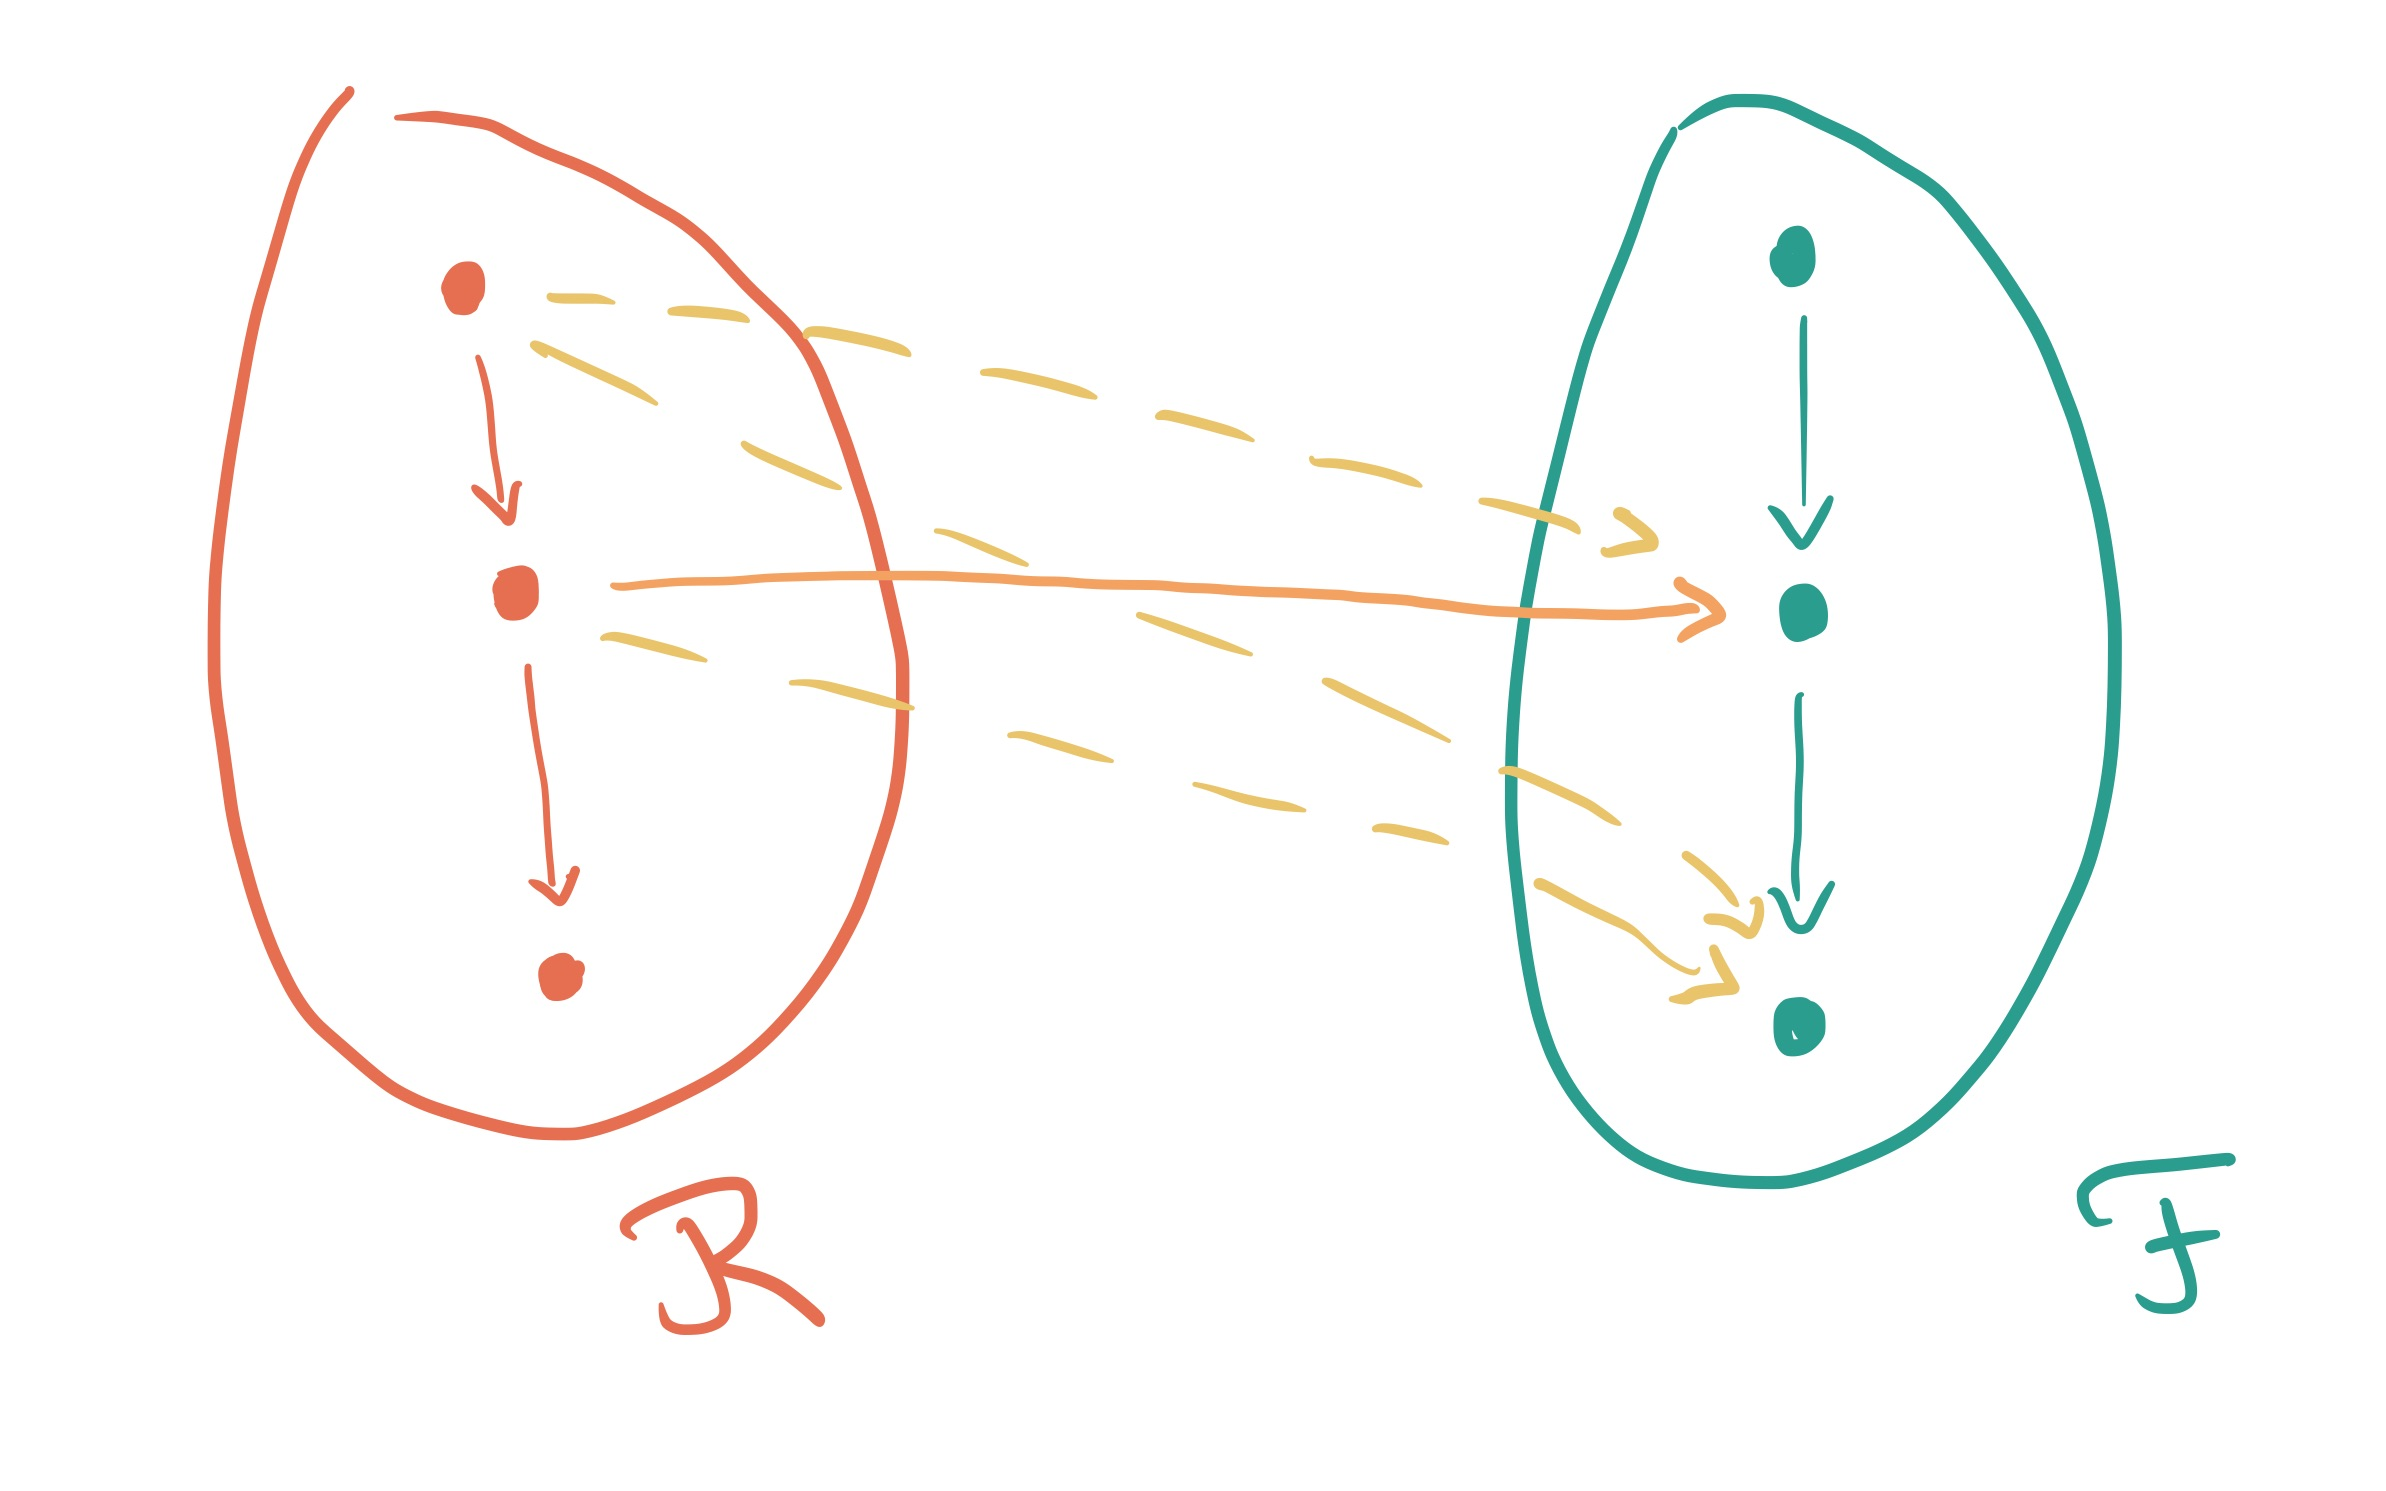
\includegraphics[width=\textwidth/2]{section2/feas_internal-1}
	\end{center}
	The orange and yellow arrows mean that a given pair is mapped to \texttt{true}. Absence of an arrow means the pair is mapped top \texttt{false}. Additionally, we may think of a feasibility relation as being generated by certain assignments. The solid orange arrow induces the dashed yellow arrows by composition with the arrows internal to both $\mc{R}$ and $\mc{F}$. 
\end{remark}

We can now define a category in which feasibility relations live.
\begin{definition}
	The category $\mathbf{DP}$ of co-design problems has posets as objects and feasibility relations as morphisms. Composition is given by profunctor compostition. Explicitly, if we have feasibility relations $\Phi: \mc{X} \xslashedrightarrow{} \mc{Y}$ and $\Psi: \mc{Y} \xslashedrightarrow{} \mc{Z}$, then
	$$ 
	\Phi \fatsemi \Psi (x,z) = \bigvee_{y \in \mc{Y}}(\Phi(x,y) \wedge \Psi(y,z)).
	$$
\end{definition}

Every feasibility relation  $\mc{R} \xslashedrightarrow{\Phi} \mc{F}$ naturally gives rise to two dual optimization problems. If we fix an $f \in \mc{F}$, then we can ask what the minimal set of resources $r \in \mc{R}$ are, such that $\Phi(r,f) = \texttt{true}$, that is $(r,f)$ is feasible. In formulae:
\begin{IEEEeqnarray*}{rCl}
	f_\text{max} & = & \text{Max} \{r \in \mc{R} \:\: |\: \Phi(r,f) = \texttt{true} \} \\ 
	& = &\{r \in \mc{R} \:\: |\: \Phi(r,f) = \texttt{true} \text{ and } \forall r': \Phi(r',f) = \mathtt{true} \wedge r \rightarrow r' \Rightarrow r=r' \}.
\end{IEEEeqnarray*}

Observe that the minimality condition implies that this set is an antichain in $\mc{R}$. Hence we get a function $h: \mc{F} \rightarrow \mathsf{A}\mc{R}$, $f \mapsto f_\text{max}$ where $\mathsf{A}\mc{R}$ denotes the set of antichains of $\mc{R}$. We can put a partial ordering on $\mathsf{A}\mc{R}$ by saying $A \leq B$ iff $\downarrow A \sub \: \downarrow B$, where $\downarrow$ denotes the lower closure operator. In our convention the lower closure of a set is all of the resources / functionalities that are `more expensive' than items in the set.

\begin{lemma}
	If all ascending chains in $\mc{R}$ are finite, then the map $h: \mc{F} \rightarrow \mathsf{A}\mc{R}$ is monotone. That is, if $f \rightarrow g$, then $\downarrow f_\text{max} \sub \: \downarrow g_\text{max}$.
\end{lemma}
\begin{proof}
	Let $f \rightarrow g$, and $x \in \: \downarrow f_\text{max}$. This means $x \rightarrow r$ for some $r \in f_\text{max}$. Because $\Phi(r,f) = \texttt{true}$ also $\Phi(x,g) = \texttt{true}$ using monotonicity in both arguments. Consider $\{s \in \mc{R} \:\: |\: x \rightarrow s  \text{ and } \Phi(s,g) = \texttt{true} \}$. This set is non-empty because it contains x itself. Moreover it has to contain a maximal element, otherwise we could build an infinite ascending chain. This maximum $m$ will be an element of $g_\text{max}$, hence we have an arrow $x \rightarrow m$, which means $x \in \downarrow g_\text{max}$
\end{proof}

\paragraph{Warning!} The map $h$ does not have to monotone in general (even if one uses upper closure or the opposite orderings). The ascending chain condition assures that one does not have arbitrarily cheap resources. To see that it is necessary consider $\mc{R} = (\mathbb{Z},\leq)$, $\mc{F} = {a \rightarrow b}$ with feasibility relation $\Psi(r,f) = \texttt{true}$ iff $f = b$ or $r \leq 0$. Then $a_\text{max} = \text{Max}\{n \in \mathbb{Z} | \Psi(r,a) = \texttt{true}\} = 0$ and $b_\text{max} = \text{Max}\{n \in \mathbb{Z} | \Psi(r,b) = \texttt{true}\} = \text{Max }\mathbb{Z} = \emptyset$. Hence $\downarrow a_\text{max} = \mathbb{Z}_{\leq 0} \nsubseteq \emptyset = \downarrow b_\text{max}$.

\subsection{Sites to Structure}

The main goal of this project is to add some of the structure of Linear Logic to the co-design framework. In principle, there are several places in the theory where one could consider implementing these concepts. Here we describe four possibilities and give some thoughts on how they may be related.
\begin{center}
	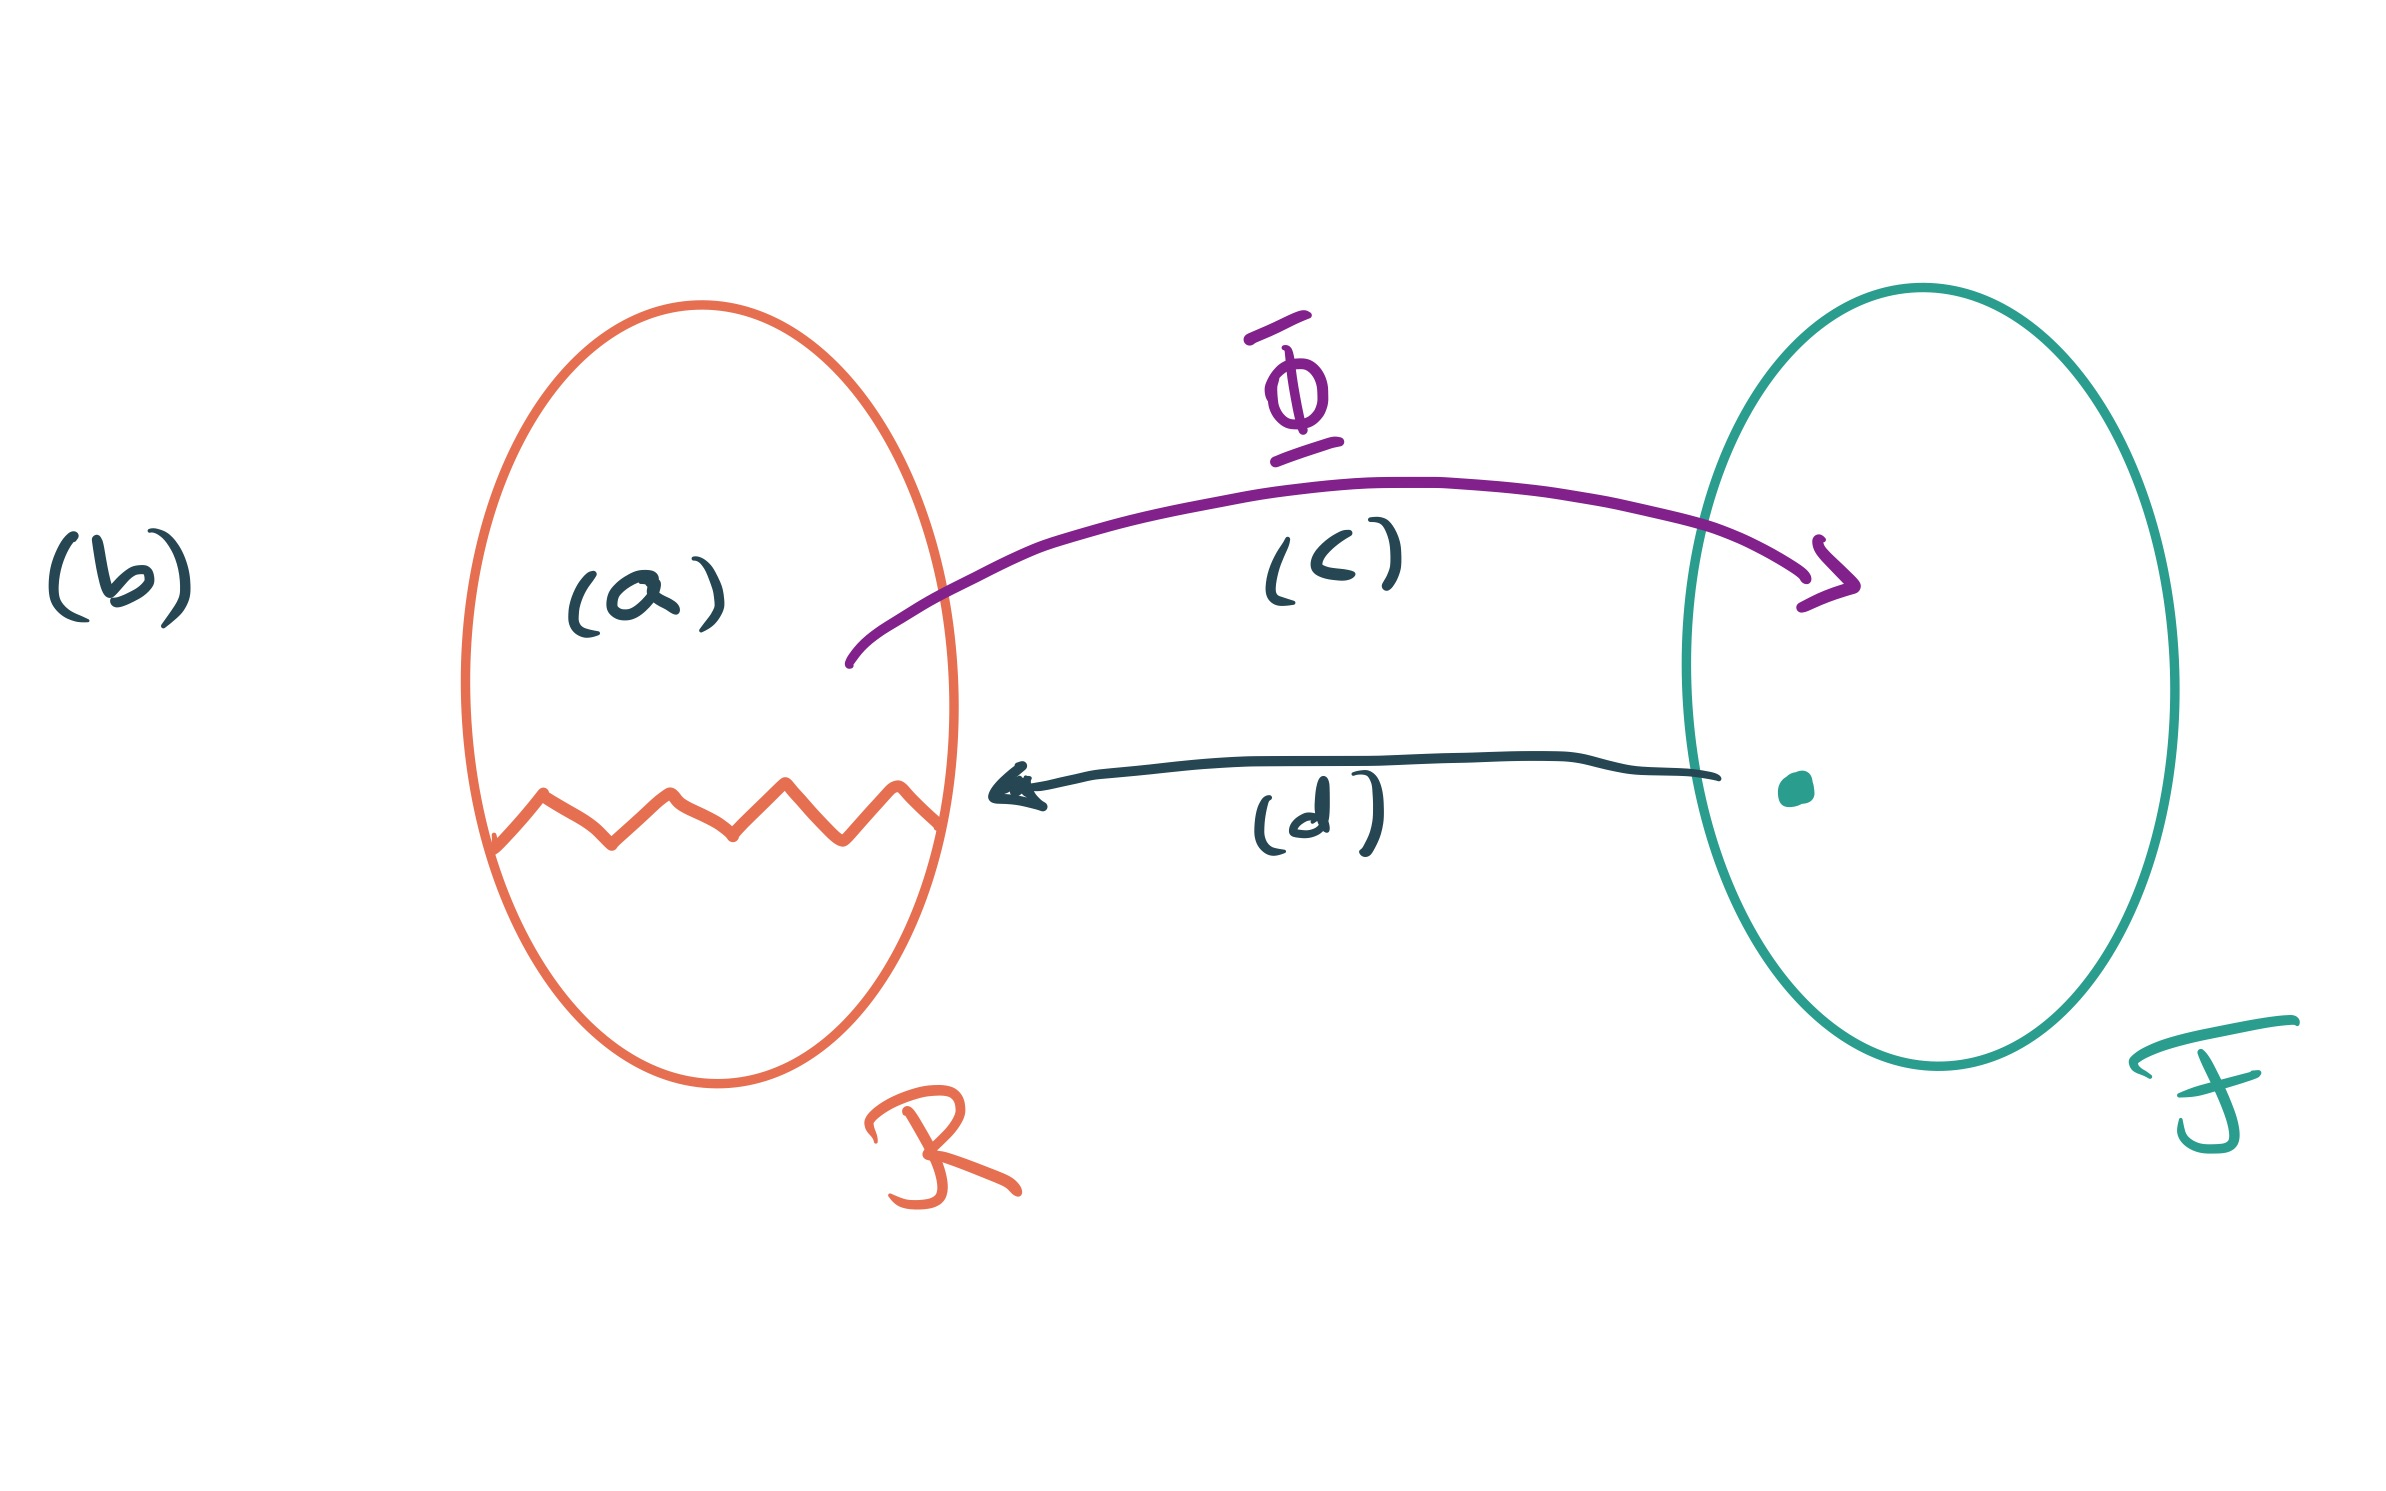
\includegraphics[width=250pt]{section2/sites_structure-1}
\end{center}

One can imagine having Linear Logic (LL) structure:
\begin{itemize}
	\item[(a)] internal to the resource / functionality posets. This would involve restricting the objects of $\mathbf{DP}$ to posets that can be viewed as models for LL.
	\item[(b)] between objects of $\mathbf{DP}$. This would involve turning $\mathbf{DP}$ into a model of LL.
	\item[(c)] within a feasibility relation. This might involve looking at monotone maps $\mc{R}^\text{op} \times \mc{F} \rightarrow \mc{V}$, where $\mc{V}$ is a model for LL.
	\item[(d)] on the queries. 
\end{itemize}

Having (b) might give (a) as well, since we can regard a poset $\mc{P}$ as the collage of trivial feasibility relations between singletons: If $a \rightarrow b$, then this may be seen as a feasibility relation $\Phi: \{a\} \xslashedrightarrow{} \{b\}$ with $\Phi(a,b) = \texttt{true}$. If we collage these together we can reconstruct $\mc{P}$. For this to work we would have to describe a multi-object collage operation, but this seems possible.

The category $\mathbf{DP}$ is compact closed, which means it forms a degenerate *-autonomous category. Hence it is already a model for classical LL. However, the 4 classical LL connectives become pairwise identified. Thus the task would be to modify $\mathbf{DP}$ in such a way, that we get distinct connectives.

Next, changing the enriching category as in (c) may also affect (b). Moreover, it will alter what type of queries are possible because there would then be more states to optimize over. On the other hand, it may be possible to complexify the types of queries that can be performed, while keeping the standard boolean feasibility relation. 

\subsection{Currying Queries}

There is an adjunction between the exponential and the cartesian product in $\mathbf{Cat}$:
$$ \Hom(\mc{C} \times \mc{D}, \mc{E}) \cong \Hom(\mc{C}, \mc{E}^\mc{D}). $$
If $\mc{P}$ and $\mc{Q}$ are posets, then so is the functor category $\mc{Q}^\mc{P}$: If $g, h:\mc{P} \rightarrow \mc{Q}$ are functors (i.e monotone maps), there is at most one natural transformation $\alpha: g \Rightarrow h$, since there is at most one morphism $\alpha_p : g(p) \rightarrow h(p)$ for each $p \in \mc{P}$. Therefore, the adjunction restricts to the subcategory $\mathbf{Pos}$ of posets. \\

Let $\mc{R}, \mc{F}$ be posets, and let $\mc{R} \xslashedrightarrow{\Phi} \mc{F}$ be a feasibility relation. Denote the lower sets of $\mc{R}$ by $\mathsf{L}\mc{R}$, where $A \leq B$ iff $A \sub B$. We claim that $\mathbf{Bool}^\mc{R^\text{op}} \cong \mathsf{L}\mc{R}$. A monotone map $h: \mc{R^\text{op}} \rightarrow \mathbf{Bool}$ is the same as a monotone map $h': \mc{R} \rightarrow \mathbf{Bool}^\text{op}$. The pre-image $L_h = h'^{-1}(\mathtt{true})$ is now a lower set: If $y \in L$ and $x \rightarrow y$, then $h'(x) \rightarrow h'(y) = \mathtt{true}$, so $h'(x) = \mathtt{true}$ since $\mathtt{true}$ is the bottom in $\mathbf{Bool}^\text{op}$. Moreover, if $g,h: \mc{R^\text{op}} \rightarrow \mathbf{Bool}$ and $g \Rightarrow h$, then $g(r) \rightarrow h(r)$ in $\mathbf{Bool}^\text{op}$ for all $r \in \mc{R}$. Hence, if $h(r) = \mathtt{true}$, then also $g(r) = \mathtt{true}$, which shows $L_h \sub L_g$, i.e.~$L_h \leq L_g$ in the lower set order. Conversely, for each lower set $L \sub \mc{R}$, we can construct an monotone map $l: \mc{R^\text{op}} \rightarrow \mathbf{Bool}$ by setting $l(x) = \mathtt{true}$ iff $l(x) \in L$. The result is monotone: $y \rightarrow x$ in $\mc{R}^\text{op}$ means $x \rightarrow y$ in $\mc{R}$. If $l(x) = \mathtt{false}$, then $l(y) = \mathtt{false}$, because $x \notin L \Rightarrow y \notin L$ by the contrapositive of the lower set property. Similarly, if $l(y) = \mathtt{true}$, then also $l(x) = \mathtt{true}$. It is immediate that both operations described are inverse. Therefore, $\mathbf{Bool}^\mc{R^\text{op}} \cong \mathsf{L}\mc{R}$.

Furthermore, if $\mc{R}$ has no infinite ascending chains, then each lower set corresponds uniquely to an antichain by taking its maximal elements. Since we order antichains by the order induced by their lower closures, we have $\mathsf{L}\mc{R} \cong \mathsf{A}\mc{R}$.

In summary, if $\mc{R}$ has no infinite ascending chains, we have the following series of isomorphisms:
\begin{IEEEeqnarray}{rCl}
	\Hom(\mc{R}^\text{op} \times \mc{F}, \mathbf{Bool}) & \cong & \Hom(\mc{F} \times \mc{R}^\text{op}, \mathbf{Bool}) \\
														& \cong & \Hom(\mc{F}, \mathbf{Bool}^\mc{R^\text{op}}) \\
														& \cong & \Hom(\mc{F}, \mathsf{L}\mc{R}) \\
														& \cong & \Hom(\mc{F}, \mathsf{A}\mc{R})
\end{IEEEeqnarray}

It follows that our feasibility relation $\Phi $ corresponds uniquely to a monotone function $h: \mc{F} \rightarrow \mathsf{A}\mc{R}$. To see what this function does, we follow the isos above. (1) sends $\Phi$ to its partial evaluations $f \mapsto \Phi(-,f)$. For each $f \in \mc{F}$, the function $\Phi(-,f)$ corresponds to the lower set 
$$\Phi(-,f)^{-1}(\mathtt{true}) = \{r \in \mc{R} \:|\: \Phi(r,f) = \mathtt{true} \}.$$ 
Taking maximal elements of this gives an antichain of resources, which are the cheapest resources which are feasible. But this is precisely the query $f_\text{max}$ described in section \ref{basic defs}. Hence we have show that querying correspond to equivalence described by the isomorphisms above, provided $\mc{R}$ fulfils the ascending chain condition.\\

We can repeat the above by swapping the roles of $\mc{F}$ and $\mc{R}$. Observe that $\mathbf{Bool}^\mc{F} \cong (\mathsf{L}\mc{F})^\text{op}$ as follows: If $h: \mc{F} \rightarrow \mathbf{Bool}$, then $h^{-1}(\mathtt{false})$ is a lower set. If $h(y) = \mathtt{false}$ and $x \rightarrow y$, then by monotonicity $h(x) \rightarrow h(y)$, so $x \in h^{-1}(\mathtt{false})$. Moreover, if $g,h: \mc{F} \rightarrow \mathbf{Bool}$ with $g \Rightarrow h$, then for each $r \in \mc{F}$, we have $g(r) \rightarrow h(r)$. Hence, if $h(r) = \mathtt{false}$, then $g(r) = \mathtt{false}$, so $h^{-1}(\mathtt{false}) \sub g^{-1}(\mathtt{false})$. This is the opposite of the usual ordering on $\mathsf{L}\mc{F}$. The inverse operation is obtained by setting $l(x) = \mathtt{false}$ iff $x$ is in the lower set. Thus $\mathbf{Bool}^\mc{F} \cong (\mathsf{L}\mc{F})^\text{op}$, as claimed.

We must now change up our isos slightly:. Assuming 	$\mc{F}$ has no infinite ascending chains:
\begin{IEEEeqnarray}{rCl}
	\Hom(\mc{R}^\text{op} \times \mc{F}, \mathbf{Bool}) & \cong & \Hom(\mc{R}^\text{op}, \mathbf{Bool}^\mc{F}) \\
	& \cong & \Hom(\mc{R}^\text{op}, (\mathsf{L}\mc{F})^\text{op}) \\
	& \cong & \Hom(\mc{R}, \mathsf{L}\mc{F}) \\
	& \cong & \Hom(\mc{R}, \mathsf{A}\mc{F})
\end{IEEEeqnarray}

The composite map sends $r \in \mc{R}$ to the antichain of the `cheapest' functionalities in $\mc{F}$ that are still infeasible.  \\ 

By swapping out lower sets for upper sets in the above, we should be able to get two more querying operation, provided the target poset fulfils a descending chain condition: One sends $f \in \mc{F}$ to the antichain of the most `expensive' resources that still make the functionality infeasible. The other sends a resource to the most `expensive' antichain of functionalities that makes the pairs feasible.

\subsection{Bool-Posets} \label{bool-pos}
We have seen above that there is a tight relation between maps into $\mathbf{Bool}$ and lower sets, upper sets, and antichains. This leads up to consider such maps as the objects of a category. 

\begin{definition} 
	A \emph{\textbf{Bool}-poset} is just a monotone map $\mc{P} \rightarrow \mathbf{Bool}$ from a poset $\mc{P}$ into $\mathbf{Bool}$. 
\end{definition}

Next we define feasibility relations between $\mathbf{Bool}$-posets.

\begin{definition} \label{def bool-pos morphism}
	A feasibility relation between $\mathbf{Bool}$-posets $\rho: \mc{R} \rightarrow \mathbf{Bool}$ and $\varphi: \mc{F} \rightarrow \mathbf{Bool}$, is a feasibility realtion $\mc{R} \xslashedrightarrow{\Phi} \mc{F}$, where for all $r \in \mc{R}$ and $f \in \mc{F}$,
	$$\Phi(r,f) = \mathtt{true} \Rightarrow \rho(r) \leq \varphi(f).$$
\end{definition}

We can express this condition in the following diagram which commutes up to a natural transformation:

\begin{center}
\begin{tikzcd}
	\mc{R} \arrow[rrd, bend left=25, ""{name=R, below}] \arrow[d, "|" marking] &  &    \\
	\mc{F} \arrow[rr, ""{name=F}]     &  & \mathbf{Bool} 
	 \arrow[Rightarrow, from=R, to=F]
\end{tikzcd}
\end{center}

\paragraph{Warning!} Requiring the condition $\varphi(f) \leq \rho(r)$ leads to the restriction that resources above a certain threshold must be mapped bellow a certain functionality threshold, which is the opposite of what we want.

\begin{lemma}
	$\mathbf{Bool}$-posets and their feasibility relationships form a category, denoted $\mathbf{Pos_{Bool}}$. Composition is given by the usual composition of feasibility relations. 
\end{lemma}

\begin{proof} 
	If $\Phi: X \xslashedrightarrow{} Y$, $\Psi: Y \xslashedrightarrow{} Z$ are feasibility relations between $\mathbf{Bool}$-posets $\xi: X \rightarrow \mathbf{Bool}$, $\upsilon: Y \rightarrow \mathbf{Bool}$ and $\zeta :Z \rightarrow \mathbf{Bool}$, then if $\Phi~\fatsemi~\Psi(x,z)$, the exists $y \in Y$ such that $\Phi(x,y)$ and $\Psi(y,z)$. Hence $\xi(x) \leq \upsilon(y)$ and $\upsilon(y) \leq \zeta(z)$, whence $\xi(x) \leq \zeta(z)$. This shows that composition is well-defined. Associativity is inherited from the composition of feasibility relations. Finally, there are identities given by the unit feasibility relation $\id: X \xslashedrightarrow{} X$, with $\id(x,y) = \mathtt{true}$ iff $x \rightarrow y \in X$. These satisfy the condition for being a morphism in $\mathbf{Pos_{Bool}}$: If $\id(x,y) = \mathtt{true}$, then $x \rightarrow y$, so $\xi (x) \leq \xi(y)$. Moreover, they are the identities for usual feasibility relations (see Fong / Spivak Lemma 4.19), so they also act that way here. 
\end{proof}

The category $\mathbf{Pos_{Bool}}$ has some interesting features, which we explore below:

\paragraph{Feasibility Relations are Objects} Since a feasibility relation $\Phi: \mc{R}^\text{op} \times \mc{F} \rightarrow \mathbf{Bool}$ is just a monotone map into $\mathbf{Bool}$, it is an object of $\mathbf{Pos_{Bool}}$. We can thus build feasibility relations between feasibility relations: If $\Psi: \mc{R'}^\text{op} \times \mc{F'} \rightarrow \mathbf{Bool}$ is another feasibility relation, a second order feasibility relation $\Phi \xslashedrightarrow{\Delta} \Psi$ would be a monotone map 
$$\Delta: (\mc{R}^\text{op} \times \mc{F})^\text{op} \times \mc{R'}^\text{op} \times \mc{F'} \rightarrow \mathbf{Bool}$$
satisfying
$$ \Delta((r,f),(r',f')) = \mathtt{true} \Rightarrow \Phi(r,f) \leq \Psi(r',f') .$$
Hence if $((r,f),(r',f'))$ is feasible, then $\Phi(r,f) \Rightarrow \Psi(r',f')$. Hence our association must preserve feasibility.

\paragraph{Limits and Colimits}

\paragraph{Inclusion of Pos}

\paragraph{Inclusion of DP}

\paragraph{Projection to DP}

\paragraph{The above form an adjunction}

\subsection{Queries in $\mathbf{Pos_{Bool}}$}

\subsubsection{Generalized Querying} \label{gen queries}
We can generalize the notion of query within $\mathbf{Pos_{Bool}}$. We can interpret an object $\varphi: \mc{F} \rightarrow \mathbf{Bool}$ as representing a poset together with a chosen lower set (resp. upper set). This is done by considering the pre-image of \texttt{false} (resp. \texttt{true}). Conversely, choosing a lower set (resp. upper set) on a poset gives an object of $\mathbf{Pos_{Bool}}$. 

Using this interpretation, let $\mc{R}, \mc{F}$ be posets representing resources and functionalities, respectively. Choose lower sets $L_\mc{R} \sub \mc{R}$ and $L_\mc{F} \sub \mc{F}$. Recall that lower sets represent resources / functionalities that closed under being more `expensive'. If the posets fulfil the ascending chain condition, we can think of the lower sets as thresholds, where we include anything more `expensive' than the elements of some antichain. 

Now observe that a morphism in  $\mathbf{Pos_{Bool}}$ is a feasibility relation $\mc{R} \xslashedrightarrow{\Phi} \mc{F}$, such that if $(r,f)$ is feasible then $\rho(r) \leq \varphi(f)$, where $\varphi(f) = \mathtt{false}$ iff $f \in L_\mc{F}$, and $\rho(r) = \mathtt{false}$ iff $r \in L_\mc{R}$. Hence, if $(r,f)$ is feasible and $f \in L_\mc{F}$, then $r \in L_\mc{R}$. Conversely, if $r \in  \mc{R} \setminus L_\mc{R}$, then $f \in f \in \mc{F} \setminus L_\mc{F}$. In our threshold interpretation this means the following for a feasible pair $(r,f)$: If $f$ lies above (or on) our threshold for functionality, then $r$ must lie above our threshold for resources. Conversely, if $r$ lies below our resource threshold, then $f$ lies below the functionality threshold.

Lets first think about varying $L_\mc{R}$. On one extreme if we let $L_\mc{R} = \mc{R}$, this would impose no restrictions whatsoever. On the other, if we choose $L_\mc{R} = \emptyset$, then only feasible pairs are allowed where $f$ lies below the functionality threshold. Now lets vary $L_\mc{F}$. If $L_\mc{F} = \mc{F}$, then only feasible pairs with $r$ above the resource threshold are allowed. If $L_\mc{F} = \emptyset$, we impose no restrictions. 

\begin{remark}
	It may seem like the variances are off here. However, suppose we had a condition that said, ``if you are above a certain resource threshold, then you are above a certain funcionality threshold''. This can't work, since if $(r,f)$ is feasible and $r$ is above the threshold, it may be that $f$ is also above the threshold, but because of monotonicity $(r,f')$ will also be feasible for any $f \rightarrow f'$. Such an $f'$ could then lie below the threshold. So our threshold would have to be trivial in order to have any feasible pairs.
\end{remark}

We can ask the following: Given some fixed feasibility relation and fixed lower set $L_\mc{F}$ in $\mc{F}$, i.e.~some lower threshold for functionality, how low do we need to set the threshold in $\mc{R}$, i.e.~how big do we need to make $L_\mc{R}$ until we get a feasibility relation that can satisfy the condition for a morphism in $\mathbf{Pos_{Bool}}$.

To see what this amounts to, lets take some feasibility relation $\Phi$ and fix $f \in \mc{F}$. We then set $L_\mc{F} = \downarrow f$. Our optimization procedure above would then yield a minimal lower set $L_\mc{R}$ in $\mc{R}$ such that if $\Phi(r,f)$ and $g \in \downarrow f$, then $r \in L_\mc{R}$. Assuming $\mc{R}$ has no infinite ascending chains, we can associate to $L_\mc{R}$ an antichain whose elements $r$ are the `cheapest' resources making $(r,f)$ feasible: The minimality on $L_\mc{R}$ means that all elements $r$ in $L_\mc{R}$ do in fact make $(r,f)$ feasible, otherwise we could have excluded them to obtain a smaller lower set. The restriction on $L_\mc{R}$ means that we have found the cheapest resources for which $f$ is feasible. If we take any element $s$ that lies strictly below the antichain, $(s,f)$ will not be feasible. For if $(s,f)$ were feasible, then $s \in L_\mc{R}$. 

In summary, we have shown that we can describe the optimization of section \ref{basic defs} in this setting. However, we can more generally query antichains of functionalities, rather than just single elements.

\subsubsection{The Generalized Query Functor}

Generalized querying as described in section \ref{gen queries} yields a contravariant functor $\mathbf{DP_\text{asc}} \rightarrow \mathbf{Pos}$, where $\mathbf{DP_\text{asc}}$ is the subcategory of $\mathbf{DP}$ where all posets satisfy the ascending chain condition. It sends a feasibility relation $\mc{R} \xslashedrightarrow{\Phi} \mc{F}$ to the monotone map $H_\Phi: \mathsf{A}\mc{F} \rightarrow \mathsf{A}\mc{R}$ which assigns each antichain in $\mc{F}$ the antichain of resources in $\mc{R}$ obtained by querying.

\textcolor{red}{Functoriality \ldots}

\subsection{Queries as Universal Objects in $\mathbf{Pos_{Bool}}$}

Recall the diagram expressing the condition for morphisms in $\mathbf{Pos_{Bool}}$.

\begin{center}
	\begin{tikzcd}
		\mc{R} \arrow[rrd, bend left=25, ""{name=R, below}] \arrow[d, "|" marking] &  &    \\
		\mc{F} \arrow[rr, ""{name=F}]     &  & \mathbf{Bool} 
		\arrow[Rightarrow, from=R, to=F]
	\end{tikzcd}
\end{center}

We can ask whether for fixed $\mc{R} \xslashedrightarrow{\Phi} \mc{F}$ and fixed $\phi: \mc{F} \rightarrow \mathbf{Bool}$, there is a universal $\rho$:  For any $\rho': \mc{R} \rightarrow \mathbf{Bool}$ which makes $\Phi$ a morphism in $\mathbf{Pos_{Bool}}$, we have $\rho'(r) \leq \rho(r)$ for all $r \in \mc{R}$. This means $\rho$ is the maximal monotone map that makes $\Phi$ a morphism in $\mathbf{Pos_{Bool}}$. 

\begin{center}
	\begin{tikzcd}
		\mc{R} \arrow[rrd, bend left=45, ""{name=R, below}] \arrow[rrd, bend right=0, "\rho" description,""{name=L, above}, ""{name=G, below}] \arrow[d, "|" marking] &  &    \\
		\mc{F} \arrow[rr, ""{name=F}]     &  & \mathbf{Bool} 
		\arrow[Rightarrow, from=R, to=L] \arrow[Rightarrow, from=G, to=F]
	\end{tikzcd}
\end{center}


Lets see what this means. We can think about $\rho$ and $\varphi$ as a lower sets $L_\rho \sub \mc{R}$ and $L_\varphi \sub \mc{F}$ in and by taking the pre-images of \texttt{false}. Because $\rho$ makes $\Phi$ a morphism in $\mathbf{Pos_{Bool}}$, if $(r,f)$ is feasible and $f \in L_\phi$, then $r \in L_\rho$. Moreover, the universality of $\rho$ makes $L_\rho$ the smallest lower set making $\Phi$ a morphism in $\mathbf{Pos_{Bool}}$. This is exactly the result of the optimization in section \ref{gen queries}. In summary, we have given a description of the process there in terms of a universal property. 

\begin{lemma}
	We can obtain the universal $\rho$ by setting $\rho(r) = \bigwedge_{\{f \:|\: \Phi(r,f)\}} \varphi(f)$
\end{lemma}
\begin{proof}
	The result is monotone: If $r \rightarrow s$ and $\rho(s) = \mathtt{false}$, then there is $f$ with $\varphi(f) = \mathtt{false}$ and $\Phi(s,f) = \mathtt{true}$. But then $\Phi(r,f) = \mathtt{true}$ by monotonicity, hence $\rho(f) = \mathtt{false}$ as well. On the other hand if $\rho(r) = \mathtt{true}$, then $\varphi(f) = \mathtt{true}$ for all $f$ satisfying $\Phi(r,f) = \mathtt{true}$. If $\rho(s)$ were \texttt{false}, then there is a $f$ with $\Phi(s,f) = \mathtt{true}$ and $\varphi(f) = \mathtt{false}$. But by monotonicity also $\Phi(r,f) = \mathtt{true}$, a contradiction. 
	
	Finally, we show that this $\rho$ is universal. First, suppose $\Phi(r,f) = \mathtt{true}$. If $\varphi(f) = \mathtt{false}$, then we have a \texttt{false} in the big wedge, so $\rho(r) = \text{false}$. Hence, $\rho$ makes $\Phi$ a morphism in $\mathbf{Pos_{Bool}}$. Suppose we have any other $\rho'$ making $\Phi$ a morphism. It is sufficient to show $\rho'(r) \Rightarrow \rho(r)$. Suppose $\rho'(r) = \mathtt{true}$. If $\rho(r) = \mathtt{false}$, then there would be $f$ such that $(r,f)$ is feasible and $\varphi(f)$ is \texttt{false}. But $(r,f)$ feasible implies that $\mathtt{true} = \rho'(r) \leq \varphi(r) = \mathtt{false}$, a contradiction. Therefore $\rho(r) = \mathtt{true}$ and we have proved universality.
\end{proof}


\subsubsection{Describing Other Queries}
The other optimization problem we can describe in this way is shown in the following diagram

\begin{center}
	\begin{tikzcd}
		\mc{R}  \arrow[rrd, bend right=0, ""{name=L, above}, ""{name=G, below}] \arrow[d, "|" marking] &  &    \\
		\mc{F} \arrow[rr,"\phi" description, ""{name=F}, ""{name = A, below}] \arrow[rr, bend right = 50, ""{name=B, above}]    &  & \mathbf{Bool} 
		 \arrow[Rightarrow, from=G, to=F] \arrow[Rightarrow, from=A, to=B]
	\end{tikzcd}
\end{center}

The univesal $\varphi$ would satisfy: For any $\varphi'$ making $\Phi$ a morphism in $\mathbf{Pos_{Bool}}$, we have $\phi \leq \phi'$. This makes the associated lower set $L_\phi$ the largest lower set making a given antichain of resources feasible.

\section{Proslice $\mc{Q}$-Categories}

The aim of this section is to generalize the construction given in \cite{Schalk2004}. In that paper, $\text{P}_F\text{-Sets}$ are constructed based on the category $\mathbf{Rel}$ of sets and relations. That construction seems to work in general for a compact closed category, whose morphisms into the valuation object are partially ordered. This setting is generalized to the category $\mathbf{Prof}(\mc{Q})$ of $\mc{Q}$-profunctors, where $\mc{Q}$ is a commutative quantale. The valuation object can then be any $\mc{Q}$-enriched category, including $\mc{Q}$ itself.

\subsection{Quantales}
The basic definitions are taken from \cite{Marsden2018}. The relation of quantales to linear logic is described in \cite{Yetter1990}.

\begin{definition}[Quantale]
	A \emph{quantale} is a complete join semilattice with a monoid structure $(\circledast, k)$ where the multiplication distributes over arbitrary joins:
	$$
	p \circledast \left( \bigvee_i q_i \right) = \bigvee_i p \circledast q_i \quad \text{ and } \quad \left( \bigvee_i p_i \right) \circledast q = \bigvee_i p_i \circledast q
	$$
	A \emph{commutative quantale} is a quantale whose underlying monoid is commutative.
\end{definition}

In the following we let $\mc{Q}$ denote a commutative quantale.

\begin{definition}[$\mc{Q}$-enriched Category]
	A $\mc{Q}$-enriched category $\mc{P}$ consist of:
	\begin{itemize}
		\item A set of \emph{objects} $\text{Ob}(\mc{P})$
		\item For each pair of objects, there is a \emph{hom object} $\mc{P}(a,b) \in \mc{Q}$ satisfying:
			\subitem{(i)} $k \leq \mc{P}(a,a)$
			\subitem{(ii)} $\mc{P}(b,c) \circledast \mc{P}(a,b) \leq \mc{P}(a,c).$
	\end{itemize}
\end{definition}

\begin{definition}[$\mc{Q}$-enriched Functor]
	If $\mc{A}$ and $\mc{B}$ are $\mc{Q}$-enriched categories, then a \emph{$\mc{Q}$-enriched functor} $F: \mc{A} \rightarrow \mc{B}$ consists of a function $$F: \text{Ob}(\mc{A}) \rightarrow \text{Ob}(\mc{B}) $$ satisfying $$ \mc{A}(a,b) \leq \mc{B}(Fa,Fb) .$$
\end{definition}

This gives us an ordinary category $\mathbf{Cat}(\mc{Q})$ whose objects are $\mc{Q}$-enriched categories and whose morphisms are $\mc{Q}$-enriched functors. \\

Because $\mc{Q}$ is thin, there can be at most one natural transformation between any two $\mc{Q}$-functors.

\begin{definition}[$\mc{Q}$-enriched Natural Transformation]
	Given parallel $\mc{Q}$-enriched functors $F,G: \mc{A} \rightarrow \mc{B}$, the presence of a \emph{$\mc{Q}$-natural transformation} $\alpha: F \rightarrow G$ simply states that for all $a \in \mc{A}$ we have
	$$
	k \leq \mc{B}(Fa,Ga).
	$$
\end{definition}

Every commutative quantale is automatically closed:

\begin{lemma} \label{closed quantale}
	Let $\mc{Q}$ be a commutative quantale. Then $- \circledast b$ has a right adjoint $b \multimap -$ given by $$b \multimap c := \bigvee_{a \circledast b \leq c} a.$$
\end{lemma}
\begin{proof}
	We regard $\mc{Q}$ as a thin ordinary category. Then $- \circledast b$ is a function $\mc{Q} \times \mc{Q} \rightarrow \mc{Q}$. Moreover, if $a \leq a'$ and $b  \leq b'$, then $a \vee a' = a'$ and $b \vee b' = b'$. Hence 
	$$a' \circledast b' = (a \vee a') \circledast (b \vee b') = (a \circledast b) \vee (a \circledast b') \vee (a' \circledast b) \vee (a' \circledast b').$$
	In particular, $a \circledast b \leq a' \circledast b'$, showing $- \circledast b$ is a functor. Its right adjoint need to satisfy the natural iso
	$$\mc{Q}(a \circledast b, c) \cong \mc{Q}(a, b \multimap c),$$ which reduces to the requirement that 
	$$a \circledast b \leq c \Leftrightarrow a \leq b \multimap c.$$
	The left-to-right implication is immediate, as by assumption $a$ appears in the join. For the right-to-left implication, suppose $a \leq \bigvee_{x \circledast b \leq c} x$. Then $$a \circledast b \leq  \left( \bigvee_{x \circledast b \leq c} x \right) \circledast b = \bigvee_{x \circledast b \leq c} x \circledast b \leq c,$$ because the join is the least upper bound. 
\end{proof}

The previous lemma implies that we can regard $\mc{Q}$ as being enriched over itself by setting $\mc{Q}(a,b) = a \multimap b$. In particular, we can can consider $\mc{Q}$-functors into $\mc{Q}$.

\begin{definition}[(Co)Presheaf]
	Let $\mc{A}$ be a $\mc{Q}$-category. A \emph{copresheaf} is a $\mc{Q}$-functor $F: \mc{A} \rightarrow \mc{Q}$. This means $F$ must satisfy
	$$
	\mc{A}(a,b) \leq F(a) \multimap F(b), \text{   or equivalently   }  \mc{A}(a,b) \circledast F(a) \leq F(b).
	$$
	A \emph{presheaf} is a $\mc{Q}$-functor $G: \mc{A}^\text{op} \rightarrow \mc{Q}$. This means $G$ must satisfy
	$$
	\mc{A}(a,b) \leq F(b) \multimap F(a), \text{   or equivalently   } \mc{A}(a,b) \circledast F(b)  \leq F(a).
	$$

\end{definition}

The monoidal structure of $\mc{Q}$ can be lifted to $\mc{Q}$-categories.
\begin{definition}[Product Category]
	Let $\mc{A}, \mc{B}$ be $\mc{Q}$-categories. Define the \emph{product category} $\mc{A} \circledast \mc{B}$ to be the $\mc{Q}$-category with objects $\text{Ob}(\mc{A}) \times \text{Ob}(\mc{B})$ and hom objects $$\mc{A} \circledast \mc{B}((a,b),(a',b')) := \mc{A}(a,a') \circledast \mc{B}(b,b').$$
\end{definition}

\begin{lemma}
	The operation $- \circledast -$ defines a bifunctor on $\mathbf{Cat}(\mc{Q})$.
\end{lemma}
\begin{proof}
	Let $\alpha: A \rightarrow B$, $\gamma: C \rightarrow D$ be $\mc{Q}$-functors. Define $(\alpha \circledast \gamma )(a,b) := (\alpha(a),\gamma(b))$. To see that this is again a $\mc{Q}$-functors, we note that 
	$$
	A(a,a') \leq B(\alpha(a),\alpha(a')) \quad \text{ and } \quad C(c,c') \leq D(\gamma(d),\gamma(d'))
	$$
	Hence, by monotonicity of $\circledast$ (see proof of Lemma \ref{closed quantale}),
	\begin{IEEEeqnarray*}{rCl}
		 (A \circledast C)(a,c)(a',c') & = & A(a,a') \circledast C(c,c')  \\
		 								&\leq& B(\alpha(a),\alpha(a')) \circledast D(\gamma(d),\gamma(d')) \\
		 								& = & (B \circledast D)(\alpha(a),\gamma(c))(\alpha(a'),\gamma(c')) \\
		 								& = &(B \circledast D)((\alpha \circledast \gamma)(a,c))((\alpha \circledast \gamma)(a',c')).
	\end{IEEEeqnarray*}
	Functoriality is immediate: 
	$$
	(\id_A \circledast \id_C)(a,c) = (\id_A(a),\id_C(c)) = (a,c) = \id_{A \circledast C}(a,c)
	$$
	$$
	((\alpha'\alpha) \circledast (\gamma'\gamma))(a,c) = (\alpha'\alpha(a),\gamma'\gamma(c)) = (\alpha' \circledast \gamma')(\alpha(a), \gamma(c)) = (\alpha' \circledast \gamma')\circ(\alpha \circledast \gamma)(a,c)
	$$
	Hence $- \circledast -$ defines a bifunctor on $\mathbf{Cat}(\mc{Q})$.
\end{proof}


\begin{definition}[Opposite Category]
	If $\mc{A}$ is a $\mc{Q}$-category, its \emph{opposite category} $\mc{A}^\text{op}$ has the same objects and hom objects $\mc{A}^\text{op}(a,a') := \mc{A}(a',a)$
\end{definition}

\begin{definition}[Unit Category]
	There is a \emph{unit $\mc{Q}$-category} $\mc{I}$ consisting of a single object and the quantale unit $k$ as its single hom object. 
\end{definition}
	
\begin{definition}[Profunctor]
	Let $\mc{A}, \mc{B}$ be $\mc{Q}$-categories. A \emph{profunctor} $R: \mc{A} \xslashedrightarrow{} \mc{B}$ is a $\mc{Q}$-functor $R: \mc{A}^\text{op} \circledast \mc{B} \rightarrow \mc{Q}$. Unravelling this definition shows that $R$ must satisfy
	$$
	\mc{A}(a',a) \circledast R(a,b) \circledast \mc{B}(b,b') \leq R(a',b').
	$$
	Given profunctors $R: \mc{A} \xslashedrightarrow{} \mc{B}$ and $S: \mc{B} \xslashedrightarrow{} \mc{C}$, we can define their composite $S \circ R: \mc{A} \xslashedrightarrow{} \mc{C}$ to be
	$$
	(S \circ R)(a,c) = \bigvee_b R(a,b) \circledast S(b,c).
	$$
	This composition is associative and has an identity given by $1_\mc{A}(a,a') := \mc{A}(a,a')$. Therefore $\mc{Q}$-profunctors form a category $\mathbf{Prof}(\mc{Q})$.
\end{definition}

\begin{lemma}
	The operation $- \circledast -$ defines a bifunctor $\mathbf{Prof}(\mc{Q})$.
\end{lemma}
\begin{proof}
	We need to specify where the tensor takes morphisms. Let $\Phi: A \xslashedrightarrow{} B$, $\Psi: C \xslashedrightarrow{} D$ be morphisms between $\mc{Q}$-categories $A,B,C$, and $D$. Define $\Phi \circledast \Psi: A \circledast C \xslashedrightarrow{} B \circledast D$ by
	$$
	\Phi \circledast \Psi ((a,c),(b,d)) := \Phi(a,b) \circledast \Psi(c,d).
	$$
	To see that this specifies a $\mc{Q}$-profunctor we write down the conditions satisfied by $\Phi$ and $\Psi$
	$$
	A(a',a) \circledast \Phi(a,b) \circledast B(b,b') \leq \Phi(a',b')
	$$
	$$
	C(c',c) \circledast \Psi(c,d) \circledast D(d,d') \leq \Psi(c',d')
	$$
	Because the operation $\circledast$ is monotone (see proof of Lemma \ref{closed quantale}), this implies
	$$
	A(a',a) \circledast	C(c',c) \circledast \Phi(a,b) \circledast \Psi(c,d) \circledast  B(b,b') \circledast D(d,d') \leq \Phi(a',b') \circledast \Psi(c',d')
	$$
	Using the definition of the product, the above is equivalent to
	\begin{IEEEeqnarray*}{r}
		(A \circledast C)((a',c'),(a,c)) \circledast (\Phi \circledast \Psi)((a,c),(b,d)) \circledast (B \circledast D)((b,d),(b',d')) \\
		\leq (\Phi \circledast \Psi)((a',c'),(b',d')),
	\end{IEEEeqnarray*}
	which is exactly the requirement we need.
	Next we turn to the functoriality requirements. It is immediate form the definitions that
	\begin{IEEEeqnarray*}{rCl}
		(\id_A \circledast \id_B)((a,b),(a',b')) &=& \id_A(a,a') \circledast \id_B(b,b') \\ 
		&=& A(a,a') \circledast B(b,b') \\
		&= & (A \circledast B)((a,b),(a',b')) \\
		&= & \id_{A \circledast B}((a,b),(a',b'))
	\end{IEEEeqnarray*}
	Moreover, if in addition $\Phi' : B \xslashedrightarrow{} X$ and $\Phi': D \xslashedrightarrow{} Y$, then
	\begin{IEEEeqnarray*}{rCl}
		(\Phi' \circ \Phi)\circledast(\Psi' \circ \Psi) ((a,c),(x,y)) 	& = & (\Phi' \circ \Phi)(a,x) \circledast (\Psi' \circ \Psi)(c,y) \\
		& = & \left(\bigvee_{b \in B} \Phi(a,b) \circledast \Phi'(b,x) \right) \circledast \left(\bigvee_{d \in D} \Psi(c,d) \circledast \Psi'(d,y) \right) \\
		& = & \bigvee_{b \in B}\bigvee_{d \in D}  \Phi(a,b) \circledast \Phi'(b,x) \circledast \Psi(c,d) \circledast \Psi'(d,y) \\
		& = & \bigvee_{(b,d) \in B \circledast D} (\Phi \circledast \Psi)((a,c),(b,d)) \circledast (\Phi' \circledast \Psi')((b,d),(x,y)) \\
		& = & (\Phi \circledast \Psi) \circ (\Phi' \circledast \Psi')  ((a,c),(x,y))
	\end{IEEEeqnarray*}
	Hence $- \circledast -$ defines a bifunctor on $\mathbf{Prof}(\mc{Q})$.
\end{proof}

\begin{proposition}
	The category $\mathbf{Prof}(\mc{Q})$ is symmetric monoidal under $- \circledast - $ with unit $\mc{I}$. Moreover it has a compact closed where each object is its own dual.
\end{proposition}
\begin{proof}
	\textcolor{red}{\ldots}
\end{proof}



\subsection{Proslice Construction}

We recall that in in the case of the $\mathbf{Bool}$-posets of section \ref{bool-pos}, we defined morphisms between $\alpha: A \rightarrow \mathbf{Bool}$ and $\beta: B \rightarrow \mathbf{Bool}$ (see \ref{def bool-pos morphism}) as $\mathbf{Bool}$-profunctors $\Phi: A \xslashedrightarrow{} B$ such that if $\Phi(a,b) = \mathtt{true}$, then $\alpha(a) \leq \beta(b)$. We can make this the following condition in $\mathbf{Bool}$: 
$$\Phi(a,b) \leq \alpha(a) \multimap \beta(b) = \mathbf{Bool}(\alpha(a), \beta(b)).$$
This allows us to generalize the condition to any $\mc{Q}$-category. Furthermore, we twist the construction by an endofunctor for added flexibility. Together this yields:

\begin{definition}[Proslice Category]
	Let $\mc{Q}$ be a quantale, $E: \mathbf{Prof}(\mc{Q}) \rightarrow \mathbf{Prof}(\mc{Q})$ be an endofunctor, and $\mc{V}$ a $\mc{Q}$-category. We define the \emph{proslice category $\mathbf{Prof}(\mc{Q}) \wr \mc{V}$ over $\mc{V}$} to be the category with
	\begin{itemize}
		\item[(i)] objects are $\mc{Q}$-functors $EA \rightarrow \mc{V}$, where $A \in \mathbf{Prof}(\mc{Q})$.
		\item[(ii)] For objects $\alpha: EA \rightarrow \mc{V}$, $\beta: EB \rightarrow \mc{V}$, morphisms are profunctors $\Phi: A \xslashedrightarrow{} B$, satisfying $$(E \Phi)(a,b) \leq \mc{V}(\alpha(a),\beta(b)).$$
	\end{itemize}
\end{definition}

\begin{proof}
	Since $E$ is an endofunctor and $\mathbf{Prof}(\mc{Q})$ a category, it suffices to check that the proslice construction is closed under identities and composition. If $\alpha(a): EA \rightarrow \mc{V}$ is a $\mc{Q}$-functor, then it satisfies $EA(a,b) \leq \mc{V}(\alpha(a),\beta(b))$. But $E \; \text{Id}_A(a,b) = EA(a,b)$, so the identity profunctor satisfies the condition to be a proslice morphism. Finally, if $A \xslashedrightarrow{\Phi} B$ and $B \xslashedrightarrow{\Psi} C$ are proslice morphisms, then $E \Phi (a,b) \leq \mc{V}(\alpha(a),\beta(b))$ and $E \Psi (b,c) \leq \mc{V}(\beta(b),\gamma(c))$. Therefore,
	\begin{IEEEeqnarray*}{rCl"s}
		 E(\Psi \circ \Phi)(a,c) & = &(E\Psi \circ E\Phi)(a,c)  & (functoriality)\\
					    		 & = & \bigvee_b E\Phi(a,b) \circledast E\Psi(b,c)  & (definition) \\
								 & \leq & \bigvee_b \mc{V}(\alpha(a),\beta(b)) \circledast \mc{V}(\beta(b),\gamma(c)) & (proslice morph.) \\
								 & \leq & \bigvee_b \mc{V}(\alpha(a),\gamma(c)) & (comp. cond.) \\
								 & = & \mc{V}(\alpha(a),\gamma(c)). &
	\end{IEEEeqnarray*}
	Hence the composite of two proslice morphisms is again proslice. 
\end{proof}

\subsubsection{Relation to Profunctor Collage}

\subsubsection{Relation to Order on Profunctors}

\subsection{Properties of $\mathbf{Prof}(\mc{Q}) \wr \mc{V}$}

\subsubsection{Tensor product}

For the following we will assume that $\mc{V}$ is a monoidal $\mc{Q}$-category.

\begin{definition}[Monoidal $\mc{Q}$-category]
	A strict symmetric \emph{monoidal $\mc{Q}$-category} is a $\mc{Q}$-category $\mc{M}$ is a monoid object in $\mathbf{Cat}(\mc{Q})$. That is, $\mc{M}$ comes equipped with a multiplication $\mc{Q}$-bifunctor $\ovee:\mc{M} \circledast \mc{M} \rightarrow \mc{M}$ and a unit $\mc{Q}$-functor $\mu: \mc{I} \rightarrow \mc{M}$ making the following diagrams commute:
	\begin{center}
	\begin{tikzcd}
		\mc{M} \circledast \mc{M} \circledast \mc{M} \arrow[r, "\mc{M} \circledast \ovee"] \arrow[d, "\ovee \circledast \mc{M}"] & \mc{M} \circledast \mc{M} \arrow[d, "\ovee"] \\
		\mc{M} \circledast \mc{M} \arrow[r, "\ovee"]                                                                             & \mc{M}                                      
	\end{tikzcd}
	\begin{tikzcd}
		\mc{M} \circledast \mc{I} \arrow[rd, "\sim"'] \arrow[r, "\mc{M} \circledast \mu"] & \mc{M} \circledast \mc{M} & \mc{I} \circledast \mc{M} \arrow[ld, "\sim"] \arrow[l, "\mu \circledast \mc{M}"'] \\
		& \mc{M}                    &                                                                                  
	\end{tikzcd}
	\end{center}	 
\end{definition}

\begin{lemma}
	If $(\mc{V}, \ovee, \mu)$ is a monoidal $\mc{Q}$-category, then $\ovee$ is monotone on hom-objects: \[ \mc{V}(v,v') \circledast \mc{V}(w,w') \leq \mc{V}(v \ovee w, v' \ovee w') \]
\end{lemma}
\begin{proof}
	This is simply because $\ovee$ is a $\mc{Q}$-functor.
\end{proof}

\begin{definition}[Oplax Functor]
	\ldots
\end{definition}

\begin{proposition}
	Let $(\mc{Q}, \circledast, k)$ be commutative quantale, and $(\mc{V}, \ovee, \mu)$ a monoidal $\mc{Q}$-category. Suppose $E: \mathbf{Prof}(\mc{Q}) \rightarrow \mathbf{Prof}(\mc{Q})$ is the extension of an oplax monoidal functor $\tilde E$ on $\mathbf{Cat}(\mc{Q})$ with natural transformation $\vartheta: E(-\circledast -) \rightarrow E(-) \circledast E(-)$, such that \textcolor{BrickRed} {$E(\Phi \circledast \Psi)(x,y) \leq (E(\Phi) \circledast E(\Psi))(\vartheta_{A,B}(x), \vartheta_{C,D}(y))$ for all $\Phi, \Psi \in \mathbf{Prof}(\mc{Q})$} (looks like it would follow from naturality of $\vartheta$). Then $\mathbf{Prof}(\mc{Q}) \wr \mc{V}$ is a symmetric monoidal category where the tensor of $\alpha: EA \rightarrow \mc{V}$ and $\beta: EB \rightarrow \mc{V}$ is given by
	$$
	E(A \circledast B) \overset{\vartheta_{A,B}}{\rightarrow} E(A) \circledast E(B) \overset{\alpha \circledast \beta}{\rightarrow} \mc{V} \circledast \mc{V} \overset{\ovee}{\rightarrow} \mc{V}.
	$$
	Written out as a composition, $\alpha \ovee \beta := \alpha\pi_1\vartheta_{A,B} \ovee \beta\pi_2\vartheta_{A,B}$.
	
	The unit $\iota$ for the tensor is given by the object
	$$
	E\mc{I} \overset{\vartheta_0}{\rightarrow} \mc{I} \overset{\mu}{\rightarrow} \mc{V},
	$$
	that is, $\iota = \mu\vartheta_0$.
	The forgetful functor $\mathbf{Prof}(\mc{Q}) \wr \mc{V} \rightarrow \mathbf{Prof}(\mc{Q})$ preserves this tensor strictly.
\end{proposition}

\begin{proof}[Proof in progress...]
 	Let $\alpha: EA \rightarrow \mc{V} , \beta: EB \rightarrow \mc{V}, \gamma: EC \rightarrow \mc{V}$, and $\delta: ED \rightarrow \mc{V}$ be objects in $\mathbf{Prof}(\mc{Q}) \wr \mc{V}$. Moreover, let $\Phi: A \xslashedrightarrow{} C$ and $\Psi: B \xslashedrightarrow{} D$ be proslice morphisms. We first show that the proposed tensor product is indeed a bifunctor.
	We observe that because $\Phi$ and $\Psi$ are proslice morphisms we have
	$$
	E \Phi(a,c) \leq \mc{V}(\alpha(a),\gamma(c)) \quad \text{ and } \quad E \Psi(b,d) \leq \mc{V}(\beta(b),\delta(d)).
	$$
	Hence,
	\begin{IEEEeqnarray*}{rCl}
		E (\Phi \circledast \Psi)(x,y)  	&\textcolor{BrickRed}{\leq}& (E \Phi \circledast E \Psi)(\vartheta_{A,B}(x),\vartheta_{C,D}(y)) \\
											& = & E\Phi(\pi_1\vartheta_{A,B}(x), \pi_1\vartheta_{C,D}(y)) \circledast E\Psi(\pi_2\vartheta_{A,B}(x), \pi_2\vartheta_{C,D}(y)) \\
											& \leq & \mc{V}(\alpha\pi_1\vartheta_{A,B}(x), \gamma\pi_1\vartheta_{C,D}(y)) \circledast \mc{V}(\beta\pi_2\vartheta_{A,B}(x), \delta\pi_2\vartheta_{C,D}(y)) \\
											& \leq & \mc{V}(\alpha\pi_1\vartheta_{A,B}(x) \ovee \beta\pi_2\vartheta_{A,B}(x), \gamma\pi_1\vartheta_{C,D}(y) \ovee  \delta\pi_2\vartheta_{C,D}(y)) \\
											& = & \mc{V}(\alpha \ovee \beta(x), \gamma \ovee \delta(y))
	\end{IEEEeqnarray*}
	showing that the image of proslice morphisms under the tensor is again proslice.
	
	Functoriality of the tensor follows from the functoriality of $E$ and $- \circledast -$ of $\mathbf{Prof}(\mc{Q})$:
	$$
	E(\id_A \circledast \id_B) = E(\id_{A \circledast B}) = \id_{E(A \circledast B)}
	$$
	$$
	E((f \circ f') \circledast (g \circ g')) = E((f \circledast g)\circ(f' \circledast g')) = E(f \circledast g) \circ E(f' \circledast g').
	$$
	It remains to define the required natural isomorphisms and check the axioms for a symmetric monoidal category. We set
	$$
	\textit{assoc}: E((A \circledast B) \circledast C) \cong E(A \circledast (B \circledast C)) 
	$$
	to be the image under $E$ of the usual natural iso for the product of categories. Similarly,
	$$\textit{right}: E(A \circledast \mc{I}) \cong E(A),\: \textit{left}: E(\mc{I} \circledast A) \cong E(A) \: \text{ and } \: \textit{swap}: E(A \circledast B) \cong E(B \circledast A)$$
	are also given as images of the usual natural isos in the symmetric monoidal category $\mathbf{Prof}(\mc{Q})$. As a consequence, the axioms are automatically fulfilled, since the requisite diagrams are the images of commuting diagrams in $\mathbf{Prof}(\mc{Q})$. \textcolor{red}{The final thing to check is that all the natural isos are in fact proslice morphisms}.
	
	 \textcolor{red}{Claim about forgetful functor}.
	
\end{proof}


\subsection{Proslice \textbf{Bool}-Categories}

We attempt to first develop the theory in the simplified setting of $\mathbf{Bool}$-enriched categories. For the following denote $\mathbf{Bool} =: \mathbb{B}$.

\begin{definition}[Proslice \textbf{Bool}-categories]
	Let $\mc{Q}$ be a commutative quantale, and $E: \mathbf{Prof}(\mathbb{B}) \rightarrow \mathbf{Prof}(\mathbb{B})$ an endofunctor. The \emph{proslice category} $\mathbf{Prof}(\mathbb{B}) \wr_E \mc{Q}$ consists of:
	\begin{itemize}
		\item[(i)] objects are monotone maps $\varphi: EP \rightarrow \mc{Q}$ 
		\item[(ii)] morphisms between $\varphi: EP \rightarrow \mc{Q}$ and $\rho: ER \rightarrow \mc{Q}$ are feasibility relations $\Phi: P \xslashedrightarrow{} R$ satisfying the \emph{proslice condition}:
		\[E\Phi(a,b) = \mathtt{true} \Rightarrow \varphi(a) \leq \rho(b). \]
	\end{itemize}
	Diagrammatically:
	\begin{center}
		\begin{tikzcd}
			EP \arrow[rrd, bend left=25, ""{name=R, below}] \arrow[d, "|" marking] &  &    \\
			ER \arrow[rr, ""{name=F}]     &  & \mc{Q} 
			\arrow[Rightarrow, from=R, to=F]
		\end{tikzcd}
	\end{center}
\end{definition}

We can define an order structure on the objects of the proslice category. Since we want the definition to cover both boolean profunctors and monotone maps, we regard both as special types of relations, and identify a relation $A \xslashedrightarrow{} B$ with an arbitrary function $A \times B \rightarrow \mathbb{B}$.

\begin{definition}
	Let $\Phi: A \xslashedrightarrow{} B$ and $\Psi: A \xslashedrightarrow{} B$ be arbitrary relations. Set $\Phi \leq \Psi$ iff for all $a \in A$ and $b,b' \in B$ we have that $\Phi(a,b) = \mathtt{true}$ and $\Psi(a,b') = \mathtt{true}$ imply $b \leq b'$. In particular, this order restricts to the pointwise order on monotone maps and hence on objects of the proslice category.
\end{definition}

We can characterize the proslice condition in terms of the aforementioned order.

\begin{lemma}\label{proslice char}
	Let $\varphi: EP \rightarrow \mc{Q}$ and $\rho: ER \rightarrow \mc{Q}$ be proslice objects. A feasibility relation $\Phi: P \xslashedrightarrow{} R$ satisfies the proslice condition if and only if $\varphi \leq \rho \circ E\Phi$.
\end{lemma}
\begin{proof}
	Suppose $\Phi$ is proslice. If $\varphi(a,b) = \mathtt{true}$ and $\rho \circ E\Phi (a,b') = \mathtt{true}$, then $\varphi(a) = b$ and there is $r \in ER$ such that $\rho(r) = b'$ and $\Phi(a,r) = \mathtt{true}$. By the proslice condition $b = \varphi(a) \leq \rho(r) = b'$.
	
	Conversely, suppose that $\varphi \leq \rho \circ E\Phi$ and $E\Phi(a,b) = \mathtt{true}$. Because $\rho$ is a function, we have $\rho(b,c) = \mathtt{true}$ for $c := \rho(b)$. Then $\rho \circ E\Phi(a,c) = \mathtt{true}$. Now for $\varphi(a) = c'$ we have $\phi(a,c') = \mathtt{true}$, so $\phi(a) = c' \leq c = \rho(b)$ by assumption. Hence $\Phi$ is proslice.
\end{proof}

This characterization can be used to obtain some lemmas for diagram pasting. In short, pre- and post-composing with monotone maps preserved the order.

\begin{lemma}[Pre-/Post-composition]\label{pasting lemma}
	Let $S, S': B \xslashedrightarrow{} C$ be feasibility relations and $R: A \rightarrow B$ $T: C \rightarrow D$ monotone maps. If $S \leq S'$, then
	\begin{itemize}
		\item[(i)] $S \circ R \leq S' \circ R$,
		\item[(ii)] $T \circ S \leq T \circ S'$. 
	\end{itemize}
 
\end{lemma} 
\begin{proof}
	Suppose $S \leq S'$. For \textit{(i)} assume that $S \circ R (a,c) = \mathtt{true}$ and $S' \circ R (a,c') = \mathtt{true}$. There are $b,b' \in B$ satisfying $R(a) = b$, $S(b,c) = \mathtt{true}$ and $R(a) = b'$, $S'(b',c') = \mathtt{true}$. But because $R$ is a function $b = b'$, so we in fact have $S(b,c) = \mathtt{true}$ and $S'(b,c') = \mathtt{true}$, which implies $c \leq c'$ since $S \leq S'$. 
	
	For \textit{(ii)} we assume that $T \circ S (b,d) = \mathtt{true}$ and $T \circ S' (b,d') = \mathtt{true}$. There are $c,c' \in C$ such that $T(c) = d$, $T(c') = d'$ and $S(b,c) = \mathtt{true}$, $S'(b,c') = \mathtt{true}$. Since $S \leq S'$, we know $c \leq c'$. Therefore by monotonicity of $T$ we have $d = T(c) \leq T(c') = d'$.
\end{proof}

The order also behaves well with respect to the cartesian product on $\mathbf{Prof}(\mathbb{B})$.

\begin{lemma}[Product] \label{product lemma}
	Let $\alpha, \alpha': A \xslashedrightarrow{} A'$, $\beta, \beta': B \xslashedrightarrow{} B'$ be feasibility relations. If $\alpha \leq \alpha'$ and $\beta \leq \beta'$, then $\alpha \times \beta \leq \alpha' \times \beta'$.
\end{lemma}
\begin{proof}
	Assume $\alpha \times \beta((a,b),(x,y)) = \mathtt{true}$ and $\alpha' \times \beta'((a,b),(x',y')) = \mathtt{true}$. By definition of the cartesian product of profunctors this means $\alpha(a,x) = \beta(b,y) = \alpha'(a,x') = \beta'(b,y') = \mathtt{true}$. Using our hypotheses that  $\alpha \leq \alpha'$ and $\beta \leq \beta'$, we obtain $x \leq x'$ and $y \leq y'$. Hence $(x,y) \leq (x',y')$, as desired.
\end{proof}

In the following we will need to choose the endofunctor on the proslice category to have a special form. We want there to be natural transformations  $\vartheta: E(- \times -) \rightarrow E(-) \times E(-)$ and $E\mathbbm{1} \rightarrow \mathbbm{1}$ whose components are monotone maps. To make the definition we observe that both $\mathbf{Cat}(\mc{Q})$ and $\mathbf{Prof}(\mc{Q})$ embed into $\mathbf{Rel_{Pos}}$, the category whose objects are posets and whose morphisms are arbitrary relations. Hence, we can formulate a mixed naturality condition there.

\begin{definition}
	An endofunctor $E$ on $\mathbf{Prof}(\mathbb{B})$ is called \emph{slicing}, if it is oplax symmetric monoidal with respect to the cartesian product, and the components of the natural transformations are monotone functions. More precisely, for any two posets $A,B \in \mathbf{Prof}(\mathbb{B})$ we want a monotone map $\vartheta_{A,B}: E(A \times B) \rightarrow E(A) \times E(B)$ in $\mathbf{Cat}(\mathbb{B}) = \mathbf{Pos}$ that makes the following diagram commute in $\mathbf{Rel_{Pos}}$:
	\begin{center}
		\begin{tikzcd}
			E(A \times B) \arrow[r, "{\vartheta_{A,B}}"] \arrow[d, "E(\Phi \times \Psi)"] & E(A)\times E(B) \arrow[d, "E\Phi \times E\Psi"] \\
			E(A' \times B') \arrow[r, "{\vartheta_{A',B'}}"]                              & E(A')\times E(B')                              
		\end{tikzcd}
	\end{center}
	We also require a monotone map $\vartheta_0 :E\mathbbm{1} \rightarrow \mathbbm{1}$.
	
	
	
\end{definition}  

\begin{theorem}[Transfer] \label{transfer theorem}
	Suppose $E$ is slicing. Then any monotone n-ary operation on $\mc{Q}$ induces a functor $\bullet: (\mathbf{Prof}(\mathbb{B}) \wr_E \mc{Q})^{\times n} \rightarrow \mathbf{Prof}(\mathbb{B}) \wr_E \mc{Q}$ as follows:
	\begin{description}
		\item[Objects] $\alpha_i : EA_i \rightarrow \mc{Q}$ are mapped to the composite
		\begin{center}
			\begin{tikzcd}
				E(A_1 \times \ldots \times A_n) \arrow[r, "{\vartheta_{A_1,\ldots,A_n}}"] & E(A_1) \times \ldots \times E(A_n) \arrow[r, "\alpha_1 \times \ldots \times \alpha_n"] & \mc{Q}^{\times n} \arrow[r, "\bullet"] & \mc{Q}
			\end{tikzcd}
		\end{center}
		where $\vartheta_{A_1,\ldots,A_n}$ denotes the iterated application of the appropriate components of the natural transformation $\vartheta$.
			
		\item[Morphisms] $E\Phi_i: EA_i \xslashedrightarrow{} EB_i$ are mapped to $E(\Phi_1 \times \ldots \times \Phi_n)$.
	\end{description}
\end{theorem}

\begin{proof}
	Let $\bullet: \mc{Q}^{\times n} \rightarrow \mc{Q}$ be the monotone n-ary operation in question. Suppose $\alpha_i: EA_i \rightarrow \mc{Q}$,  $\beta_i: EB_i \rightarrow \mc{Q}$ are proslice objects, and $\Phi_i: A_i \xslashedrightarrow{} B_i$ proslice morphisms, for $1 \leq i \leq n$. The proslice condition, $\alpha_i \leq \beta_i \circ E\Phi_i$ implies $\alpha_1 \times \ldots \times \alpha_n \leq \beta_1 \circ E \Phi_1 \times \ldots \times \beta_n \circ E \Phi_n$ by lemma \ref{product lemma}. Because $\times$ is a functor, \[ \beta_1 \circ E \Phi_1 \times \ldots \times \beta_n \circ E \Phi_n =  (\beta_1 \times \ldots \times \beta_n) \circ (E\Phi_1 \times \ldots \times E\Phi_n). \] 
	
	By appending the relevant iterated components of the natural transformation $\vartheta$, we get the following diagram, where the left square commutes by naturality.
	\begin{center}
		\begin{tikzcd}
			E(A_1 \times \ldots \times A_n) \arrow[r, "{\vartheta_{A_1,\ldots,A_n}}"] \arrow[dd, "E(\Phi_1 \times \ldots \times \Phi_n)"] & E(A_1) \times \ldots \times E(A_n) \arrow[rd, "\alpha_1 \times \ldots \times \alpha_n"] \arrow[dd, "E\Phi_1 \times \ldots \times E\Phi_n"] &                                            &            \\
			&                                                                                                                                            & \mc{Q}^{\times n} \arrow[r, "\bullet"] & \mc{Q} \\
			E(B_1 \times \ldots \times B_n) \arrow[r, "{\vartheta_{B_1,\ldots,B_n}}"]                                                     & E(B_1) \times \ldots \times E(B_n) \arrow[ru, "\beta_1 \times \ldots \times \beta_n"']                                                     &                                            &           
		\end{tikzcd}
	\end{center}
	By using pre-composition lemma \ref{pasting lemma} and the commutativity of the square, we obtain
	\begin{IEEEeqnarray*}{rCl}
		(\alpha_1 \times \ldots \times \alpha_n) \circ \vartheta_{A_1,\ldots,A_n} &\leq& (\beta_1 \times \ldots \times \beta_n) \circ (E\Phi_1 \times \ldots \times E\Phi_n) \circ \vartheta_{A_1,\ldots,A_n} \\
			& = & (\beta_1 \times \ldots \times \beta_n) \circ \vartheta_{B_1,\ldots,B_n} \circ E(\Phi_1 \times \ldots \times \Phi_n).
	\end{IEEEeqnarray*}
	By post-composition, again using lemma \ref{pasting lemma},
	\[\bullet [(\alpha_1 \times \ldots \times \alpha_n) \circ \vartheta_{A_1,\ldots,A_n}]  \leq \bullet [(\beta_1 \times \ldots \times \beta_n) \circ \vartheta_{B_1,\ldots,B_n} \circ E(\Phi_1 \times \ldots \times \Phi_n)]. \]
	Therefore, $E(\Phi_1 \times \ldots \times \Phi_n)$ is proslice with respect to the induced operation. Finally, functoriality follows from that of $\times$ and $E$: 
	\begin{IEEEeqnarray*}{rCl}
	E(\Psi_1 \Phi_1 \times \ldots \times \Psi_n\Phi_n) &= &E((\Psi_1 \times \ldots \times \Psi_n)\circ(\Phi_1 \times \ldots \times \Phi_n)) \\ & =&  E(\Psi_1 \times \ldots \times \Psi_n) \circ E(\Phi_1 \times \ldots \times \Phi_n)	
	\end{IEEEeqnarray*}
	and
	\[E(\id_{A_1} \times \ldots \times \id_{A_n}) = E(\id_{A_1 \times \ldots \times A_n}) = \id_{E(A_1 \times \ldots \times A_n)}.\]
	
\end{proof}

\begin{remark}
	Observe that the above proof also works for any monoidal product $\otimes$ on $\mathbf{Prof}(\mathbb{B})$ and operation $\mc{Q}^{\otimes n} \rightarrow \mc{Q}$.
\end{remark}

Our goal is now to transfer the structure of the quantale $\mc{Q}$ (which we will eventually choose to be *-autonomous) to the proslice category $\mathbf{Prof}(\mathbb{B}) \wr_E \mc{Q}$. The transfer theorem \ref{transfer theorem} tells us that we will get appropriate functors on the proslice category for each operation on $\mc{Q}$. However, we will need to check that the induced operations also satisfy the requisite properties. We start with the monoidal product. 

\subsubsection{Symmetric Monoidal Structure}

\begin{proposition}
	Let $(\mc{Q},\otimes, k)$ be a commutative quantale and $E$ slicing. Then $\mathbf{Prof}(\mathbb{B}) \wr_E \mc{Q}$ is a symmetric monoidal category with respect to the bifunctor induced by $\otimes$.
\end{proposition} 
\begin{proof}
	By the transfer theorem \ref{transfer theorem}, we know that we have a bifunctor $\otimes$ on $\mathbf{Prof}(\mathbb{B}) \wr_E \mc{Q}$. We need to show that this satisfies the axioms for a SMC. The required natural isomorphisms will be inherited from those that turn the cartesian product into a symmetric monoial structure on $\mathbf{Prof}(\mathbb{B})$. These are 
	\[\mathit{assoc}: (A \times B) \times C \rightarrow  A \times (B \times C), \]
	\[\mathit{left}: \mathbbm{1} \times A \rightarrow A, \]
	\[\mathit{right}: A \times \mathbbm{1} \rightarrow A, \]
	\[\mathit{swap}: A \times B \rightarrow B \times A. \]
	which are the appropriate profunctors induced by the corresponding functions in $\mathbf{Set}$. For the proslice category, we take the images of the above natural isomorphisms under the functor $E$. This process preserves naturality and the commutativity of the requisite diagrams, since morphisms in the proslice category are just special morphisms in $\mathbf{Prof}(\mathbb{B})$. The only thing to check is that the compoents of our natural transformations actually lie in the proslice category, that is that they fulfil the proslice condition. This can be seen from the following commutative diagrams, where the top and bottom paths are the proslice objects obtained by the induced operation. The fact that they commute means that we in particular have the inequality of relations that characterizes proslice morphisms (see lemma \ref{proslice char}).
	
	We start with associativity:
	\begin{center}
		\begin{tikzcd}
			E((A \times B) \times C) \arrow[d, "E(\mathit{assoc})"] \arrow[r, "{\vartheta_{A,B}\vartheta_{(A \times B),C}}"] & (E(A) \times E(B)) \times E(C) \arrow[r, "(\alpha \times \beta) \times \gamma"] \arrow[d, "\mathit{assoc}"] & (\mc{Q} \times \mc{Q}) \times \mc{Q}  \arrow[d, "\mathit{assoc}"] \arrow[rd, "\otimes \text{ twice}"] &            \\
			E(A \times (B \times C)) \arrow[r, "{\vartheta_{B,C} \vartheta_{A,(B \times C)}}"']                             & E(A) \times (E(B) \times E(C)) \arrow[r, "\alpha \times (\beta \times \gamma)"']                            & \mc{Q} \times (\mc{Q} \times \mc{Q} ) \arrow[r, "\otimes \text{ twice}"']                             & \mc{Q}
		\end{tikzcd}
	\end{center}
	The leftmost square commutes by the associativity requirement for the oplax monoidal functor $E$, the middle square commutes by the naturality of $\mathit{assoc}$, and the rightmost triangle commutes because it is the image of the associativity diagram for $\mc{Q}$ in $\mathbf{Pos}$.
	
	The diagram for the left unitor is:
	\begin{center}
		\begin{tikzcd}
			E(\mathbbm{1} \times A) \arrow[rd, "E(\mathit{left})"'] \arrow[r, "{\vartheta_0 \vartheta_{\mathbbm{1},A}}"] & \mathbbm{1} \times E(A) \arrow[r, "\mathbbm{1} \times \alpha"] \arrow[d, "\mathit{left}"] & \mathbbm{1} \times \mc{Q} \arrow[r, "k \times \mc{Q}"] \arrow[d, "\mathit{left}"] & \mc{Q} \times \mc{Q} \arrow[ld, "\otimes"] \\
			& E(A) \arrow[r, "\alpha"]                                                                  & \mc{Q}                                                                                &                                                   
		\end{tikzcd}
	\end{center}
	The left triangle communtes by the axioms for an oplax monoidal functor, the middle square by naturality of $\mathit{left}$, and the right triangle because of the unit law for $\mc{Q}$. The diagram for the right unitor is analogous.
	
	Finally, for commutativity we have
	\begin{center}
			\begin{tikzcd}
			E(A \times B) \arrow[d, "E(\mathit{swap})"] \arrow[r] & E(A) \times E(B) \arrow[d, "\mathit{swap}"] \arrow[r] & \mc{Q} \times \mc{Q} \arrow[d, "\mathit{swap}"] \arrow[rd, "\otimes"] &            \\
			E(B \times A) \arrow[r]                               & E(B) \times E(A) \arrow[r]                            & \mc{Q} \times \mc{Q} \arrow[r, "\otimes"]                             & \mc{Q}
		\end{tikzcd}
	\end{center}
	where the left square commutes because $E$ is symmetric oplax monoidal, the middle by naturality of $\mathit{swap}$, and the right triangle by commutativity of $\mc{Q}$.
\end{proof}


\section{Bundles}

\subsection{The Setting}

For the moment we will forget about resources and functionalities and instead just consider a preorder of things. An arrow $a \rightarrow b$ expresses the fact that if I have $a$, then I can obtain $b$ from it. We imagine this as a process of instant conversion. 

In this setting we can imagine bundling things together. Such a bundle unites a collection of things to a whole. The type of bundle dictates how we are able to interact with the things therein. These interactions are characterized by what things we can obtain using the bundles and from what things we can obtain a given bundle.

We will enforce resource conservation on the bundles, meaning that we can obtain each item occurring in the bundle at most once. Conversely, if the bundle make some resources available, we are stuck with them and can't just throw them away.

\subsection{Agnostic Choice}
To start with we will assume our bundles only track availability and unavailability of things. They will be agnostic to temporal, causal, spacial, or similar features. The bundles can nonetheless create some forms of dependency between the things. 

\subsubsection{2-Bundles}
Here are all the bundles of two things $a,b$ I can think of in this case:
\begin{description}
	\item[Both(a,b)] You have both $a,b$ at the same time and can use both freely in any order.
	\item[Either(a,b)] You can choose between either having $a$ or having $b$.
	\item[Maybe(a,b)] You have either $a$ or $b$, but you don't know in advance which one. When using the bundle, it will give you either $a$ or $b$.
	\item[BombL(a,b)] Using $a$ will destroy $b$, but not vice versa. This is equivalent to $\mathsf{Either}(a,\mathsf{Both}(a,b))$.
\end{description}

We could be tempted to also introduce an ordered pair $\mathsf{Before}(a,b)$ expressing the fact that we have both $a,b$, but in a set order (temporal, spacial, causal). Our assumption that the bundles are agnostic to these features implies $\mathsf{Before}(a,b) = \mathsf{Before}(b,a)$, regardless of how we interpret the ordering. Note that in any case \[\mathsf{Both}(a,b) = \mathsf{Either}(\mathsf{Before}(a,b), \mathsf{Before}(b,a))). \]

Observe also that asymmetric dependence with respect to availability is expressed by $\mathsf{BombL}(a,b)$ and can be expressed in terms of $\mathsf{Both}$ and $\mathsf{Either}$.

Finally, note we distinguish two modes of choice, free and forced. This corresponds to two agents. In principle, we could establish more complex forms of choice by considering agents with (possibly interrelated) knowledge pools. Our situation corresponds to two agents (me and my opponent) with no shared knowledge. Specifically, $\mathsf{Either}(a,b) \rightarrow \mathsf{Maybe}(a,b)$, from my perspective, but not the other way around. From my opponents perspective, the situation is reversed.   

\subsubsection{n-Bundles}
Lets turn to bundles of higher arity. For example there could be a general bundle containing $n$ things, some of which you can choose freely, and some of which will be chosen for you. We can express this using the elementary n-bundles $\mathsf{Either}(a_1,\ldots,a_n)$, expressing a single free choice from $n$ elements and $\mathsf{Maybe}(a_1,\ldots,a_n)$, expressing a single forced choice from $n$ elements. 

For example, a bundle of 3 things with a forced choice followed by a free choice is given by 
\[\mathsf{Maybe}( \mathsf{Either}(\mathsf{Both}(a,b), \mathsf{Both}(a,c)), \mathsf{Either}(\mathsf{Both}(b,a), \mathsf{Both}(b,c)), \mathsf{Either}(\mathsf{Both}(c,a), \mathsf{Both}(c,b)))\]
This can be seen by drawing a tree of possibilities.

On the other hand if we have a free choice followed by a forced choice then we get the expression
\[\mathsf{Either}( 
\mathsf{Maybe}(\mathsf{Both}(a,b), \mathsf{Both}(a,c)), 
\mathsf{Maybe}(\mathsf{Both}(b,a), \mathsf{Both}(b,c)),
\mathsf{Maybe}(\mathsf{Both}(c,a), \mathsf{Both}(c,b))
)
\]

This begs the question of whether

\[\mathsf{Maybe}( \mathsf{Either}(X), \ldots, \mathsf{Either}(Y)) \stackrel{?}{=} \mathsf{Either}( \mathsf{Maybe}(X), \ldots, \mathsf{Maybe}(Y)). 
\]

In words, this is asking whether it matters if I can freely choose between uncertain outcomes or whether it is uncertain which free choice I will be able to make.  

Observe that in any case

\[\mathsf{Either}(\mathsf{Both}(a,b), \mathsf{Both}(a,c)) 
= \mathsf{Both}(a,\mathsf{Either}(b,c))
\]

\[ \mathsf{Maybe}(\mathsf{Both}(a,b), \mathsf{Both}(a,c)) 
= \mathsf{Both}(a,\mathsf{Maybe}(b,c)) \]

So we can reduce the first expression to

\[
\mathsf{Maybe}( \mathsf{Both}(a,\mathsf{Either}(b,c)), \mathsf{Both}(b,\mathsf{Either}(a,c)), \mathsf{Both}(c,\mathsf{Either}(a,b)))
\]

The second expression reduces to

\[
\mathsf{Either}( \mathsf{Both}(a,\mathsf{Maybe}(b,c)), \mathsf{Both}(b,\mathsf{Maybe}(a,c)), \mathsf{Both}(c,\mathsf{Maybe}(a,b)))
\]

In the example of choosing from $[a,b,c]$ it seems like the distinction is immaterial, as long as there is no dependency between $a,b,c$. In both cases I can guarantee only one resource. If there is some dependency, things may be more complicated. Suppose $\mathsf{Both}(a,b)$ is highly desirable, but $\mathsf{Both}(a,c)$ is catastrophic. All other outcomes are neutral. If you had a free choice first, you wouldn't want to choose $a$, because, then the catastrophic outcome might be realized by the forced choice. So in this case, you would always end up with a neutral outcome, if you want to avoid catastophe at all costs. On the other hand, if the forced choice was first, there is a chance you get $a$ and are able to realize the desirable outcome. Moreover, you can always avoid catastrophe.   

This could be visualized by two agents each attempting to satisfy a list of preferences by adding items to a common pool. Depending on what types of items appear on the list, it might make a difference in what order they proceed. However, it seems that a difference only manifests if they have compound items on their lists. 

\subsubsection{Substitution Rules}
We want to extend the obtaining relation $a \rightarrow b$ to bundles. We do this via the following substitution rules:
\begin{itemize}
	\item If $a \rightarrow x$ and you have $\mathsf{Both}(a,b)$, then you can get $\mathsf{Both}(x,b)$
	\item If $a \rightarrow x$ and you have $\mathsf{Either}(a,b)$, then you can get $\mathsf{Either}(x,b)$.
	\item If I have $\mathsf{Either}(a,b)$, I can obtain $a$
	\item If  $a \rightarrow x$, and you have $\mathsf{Maybe}(a,b)$, then you can get $\mathsf{Maybe}(x,b) $.
	\item If I have $a$, I can obtain $\mathsf{Maybe}(a,b)$
\end{itemize}

Moreover, we have the following simplification rules:
\begin{itemize}
	\item $\mathsf{Either}(a,a) = a = \mathsf{Maybe}(a,a)$
\end{itemize}

\subsubsection{Debt}
We can introduce a notion of debt by saying that for a resource $a$, $\neg a$ signifies that I owe an $a$. If $a \rightarrow b$, then $\neg b \rightarrow \neg a$. Assuming two parties, $\neg\neg a=a$. If $\mathsf{Maybe}$ is uncertain because it is the choice of my opponent, then $\neg \mathsf{Either}(a,b) = \mathsf{Maybe}(\neg a, \neg b)$. Equivalently, thinking in terms of unknowns, if I owe a $\mathsf{Maybe}(a,b)$, then I can choose to provide either $a$, or $b$. That is $\neg \mathsf{Maybe}(a,b) = \mathsf{Either}(\neg a, \neg b)$.

Finally, lets think about how debt interacts with $\mathsf{Both}$. It seems that owing both $a$ and $b$ independently can be expressed as $\mathsf{Both}(\neg a, \neg b)$. On the other hand $\neg \mathsf{Both}(a, b)$ would mean owing independent $a$ and $b$. It is hard to find a difference between these two formulations. Furthermore we should have $\mathsf{Both}(a, \neg a) \rightarrow [ \phantom{n}]$ and $[ \phantom{n}] \rightarrow \mathsf{Both}(a, \neg a)$.

\subsubsection{Free Bundles}

Let $\mathcal{P}$ be a countable preorder expressing obtainability. Form $\mathbf{Bundle}(\mathcal{P})$ by adding all finite expressions obtainable by $\neg$, $\mathsf{Both}$, $\mathsf{Either}$, and $\mathsf{Maybe}$, along with all arrows obtainable from the substitution rules. We wish to include also the empty expression $[ \phantom{n} ]$, which acts as the unit for $\mathsf{Both}$.

\begin{proposition} $\mathbf{Bundle}(\mathcal{P})$ is compact closed with all finite non-empty meets and joins.
\end{proposition}

\begin{proof} Multiplication is given by $\mathsf{Both}$, which is an endofunctor because of the substitution rules. Moreover, we noted above that have $\mathsf{Both}(a, \neg a) \rightarrow [ \phantom{n}]$ and $[ \phantom{n}] \rightarrow \mathsf{Both}(a, \neg a)$. The yanking equations are trivially satisfied because we are dealing with a preorder. 

Finite joins are given by $\mathsf{Maybe}$:
\[a_1 \vee a_2 = \mathsf{Maybe}(a_1,a_2)\]
We have injections $a_i \rightarrow \mathsf{Maybe}(a_1,a_2)$. Suppose $a_i \rightarrow t$ for $i=1,2$. Assume I have $\mathsf{Maybe}(a_1,a_2)$ then by two substitutions I can get $\mathsf{Maybe}(t,t) = t$. Hence $\mathsf{Maybe}(a_1,a_2) \rightarrow t$.

In a similar manner, finite meets are given by $\mathsf{Either}$.
\end{proof}

\paragraph{Warning} It is important that this compact closed preorder not have all finite meets and joins, as otherwise they would coincide by the paper of Robin Houston \cite{Houston2006}.  For example, if you had top $\top$ and bottom $\bot$, then $\mathsf{Both}(\top,\bot) \cong \bot$, because having an additional copy of $\top$ doesn't make any difference if you have the universal resource $\bot$. On the other hand, by negation and symmetry, $\top = \neg \bot \cong \neg \mathsf{Both}(\top,\bot) = \mathsf{Both}(\neg \top, \neg \bot) = \mathsf{Both}(\top,\bot)$. Hence $\top = \bot$, which in particular has the consequence that $a \cong b$ for any $a,b$, meaning any $a$ would be obtainable from any $b$. 


\subsubsection{Extending Feasibility Relations to Bundles}
Suppose we are given preorders $\mc{R}$ and $\mc{F}$, with a feasibility relation $\Phi: \mc{R} \xslashedrightarrow{} \mc{F}$. We may then extend $\Phi$ to a feasibility relation $\bar\Phi: \mathbf{Bundle}(\mc{R}) \xslashedrightarrow{} \mathbf{Bundle}(\mc{F})$ as follows.

We view $\mathbf{Bundle}(X)$ as an iterated construction starting with $X_0 = X$. Define 
$$\both(Y) = \{\both(x,y) \: | \: x,y, \in X\},$$
$$\maybe(Y) = \{\maybe(x,y) \: | \: x,y, \in X\},$$
$$\either(Y) = \{\either(x,y) \: | \: x,y, \in X\},$$
where in each case we enforce $\mathsf{Op}(a,b) = \mathsf{Op}(b,a)$ for $\mathsf{Op} \in \{\both, \maybe, \either \}$.

Then set $$X_{i+1} = X_i \cup \both(X_i) \cup \maybe(X_i) \cup \either(X_i).$$ Finally, $$\mathbf{Bundle}(X) = \bigcup_{i=0}^{\infty} X_i,$$
and add arrows according to the preorder generated by the substitution, introduction, and elimination rules.

We can now extend $\Phi$ in a stepwise fashion. Suppose we have extended $\Phi$ to a feasibility relation $\Phi_i: \mc{R}_i \xslashedrightarrow{} \mc{F}_i$. Extend this to $\Phi_{i+1}: \mc{R}_{i+1} \xslashedrightarrow{} \mc{F}_{i+1}$ as follows. For $(r,f) \in \mc{R}_i^{\text{op}} \times \mc{F}_i$ set 
$$\Phi_{i+1}(r,f) \Leftrightarrow \Phi_i(r,f)$$ 
$$\Phi_{i+1}(\neg r, \neg f)  \Leftrightarrow \neg \Phi_i(r,f),$$
$$\Phi_{i+1}(\both(r_1,r_2),\both(f_1,f_2)) \Leftrightarrow (\Phi_i(r_1,f_1) \wedge \Phi_i(r_2,f_2)) \vee (\Phi_i(r_1,f_2) \wedge \Phi_i(r_2,f_1))$$
$$\Phi_{i+1}(\either(r_1,r_2),\maybe(f_1,f_2)) \Leftrightarrow \bigvee_{l,k \in \{1,2\}}\Phi_i(r_l,f_k) , $$
$$\Phi_{i+1}(\maybe(r_1,r_2),\either(f_1,f_2)) \Leftrightarrow \bigwedge_{l,k \in \{1,2\}}\Phi_i(r_l,f_k). $$

We now need to show that this assignment makes $\Phi_{i+1}$ a feasibility relation, provided that $\Phi_i$ is a feasibility relation. By assumption, monotonicity is guaranteed on terms up to complexity $i$. Because the arrows in $\mc{R}_{i+1}, \mc{F}_{i+1}$ are generated by the substitution, elimination, and introduction rules, it is sufficient to check monotonicity for these elementary cases.

We check the extended assignments for monotonicity:

\paragraph{($\Phi_{i+1}(r,f) \Leftrightarrow \Phi_i(r,f)$)} Suppose $\Phi_{i+1}(r,f)$ and $x \rightarrow r$, $f \rightarrow y$ elementary. If $x$ or $y$ have complexity $i$, we are covered by the induction hypothesis. Otherwise $x = \either(r,s)$ and $y = \maybe(f,g)$. By the fourth rule we have $\Phi_{i+1}(\either(r,s),\maybe(f,g))$, as desired.

\paragraph{($\neg$)} Suppose $\Phi_{i+1}(\neg r, \neg f)$ and $x \rightarrow \neg r$, $\neg f \rightarrow y$ elementary. Then $x = \neg s$ for $r \rightarrow s$ and $y = \neg g$ for $g \rightarrow f$. Since $\Phi_{i+1}(\neg r, \neg f)$, we know $\neg \Phi_i(r,f)$. This implies $\neg \Phi_i(s,g)$, since $\Phi_i$ monotone. Hence $\Phi_{i+1}(\neg s, \neg g)$, that is $\Phi_{i+1}(x,y)$.

\paragraph{($\both$)} Suppose $\Phi_{i+1}(\both(r_1,r_2),\both(f_1,f_2))$ and $x \rightarrow \both(r_1,r_2)$, $\both(f_1,f_2) \rightarrow y$ elementary. Then $x = \both(s_1,s_2)$ and $y = \both(g_1,g_2)$. Thus by elementarity $s_1 \rightarrow r_1$, $s_2 \rightarrow r_2$ and $f_1 \rightarrow g_1$, $f_2 \rightarrow g_2$. Our assumption $\Phi_{i+1}(\both(r_1,r_2),\both(f_1,f_2))$ implies $(\Phi_i(r_1,f_1) \wedge \Phi_i(r_2,f_2))$ or $(\Phi(r_1,f_2) \wedge \Phi(r_2,f_1))$. Hence by monotonicity we get $(\Phi_i(s_1,g_1) \wedge \Phi_i(s_2,g_2))$ or $(\Phi(s_1,g_2) \wedge \Phi(s_2,g_1))$. This means $\Phi_{i+1}(\both(s_1,s_2),\both(g_1,g_2))$, as desired.

\paragraph{($\maybe$ right)} Suppose $\Phi_{i+1}(\either(r_1,r_2),\maybe(f_1,f_2))$ and $x \rightarrow \either(r_1,r_2)$, $\maybe(f_1,f_2) \rightarrow y$ elementary. Then $x = \either(s_1,s_2)$ and $y = \maybe(g_1,g_2)$ with $f_1 \rightarrow g_1$, $f_2 \rightarrow g_2$ and $s_1 \rightarrow r_1$,$s_2 \rightarrow r_2$. By assumption $\Phi_i(r_l,f_k)$ for some $l,k \in \{1,2\}$ with $l \neq k$ so $\Phi_i(s_l,g_k)$. Hence $\Phi_{i+1}(\either(s_1,s_2),\maybe(g_1,g_2))$.

\paragraph{($\maybe$ left)} Suppose $\Phi_{i+1}(\maybe(r_1,r_2),\either(f_1,f_2))$ and $x \rightarrow \maybe(r_1,r_2)$, $\either(f_1,f_2) \rightarrow y$ elementary. Then $x \in \{r_1,r_2\}$ and $y \in \{f_1,f_2\}$. By assumption $\Phi_i(r_l,f_k)$ for all $l,k \in \{1,2\}$ with $l \neq k$. So in all cases $\Phi_{i+1}(r_l,f_k) = \Phi_{i}(r_l,f_k)$.

This shows that $\Phi_{i+1}$ is again a feasibility relation. Observe that in the proof we only needed the operation for defining ($\both$) to be monotone on $\mathbf{Bool}$, while in the case of negation we used the fact that $\mathbf{Bool}$ has only two values, and in the case of ($\maybe$ left) we needed a conjunction. We needed the ($\maybe$ left) rule to be a disjunction, in order to get monotonicity for the elimination rules.

Now, by induction on $i$, we can extend a feasibility relation $\Phi: \mc{R} \xslashedrightarrow{} \mc{F}$ to $\Phi_\infty: \mathbf{Bundle}(\mc{R}) \xslashedrightarrow{} \mathbf{Bundle}(\mc{F})$, as we intended.

\subsubsection{Functoriality}

\subsubsection{Relation to Queries}
The construction above gives us formulae for queries. Let  $\Phi: \mc{R} \xslashedrightarrow{} \mc{F}$. First fix a resources $r_1,r_2 \in \mathbf{Bundle}(\mc{R})$ and consider $h(r) = \{f \in \mathbf{Bundle}(\mc{F}) \: | \: \Phi_\infty(r,f)\}$. 

If $f \in h(r_1) \cup h(r_2)$, then there are $i,j$ such that $\Phi_i(r_1,f)$ or $\Phi_j(r_2,f)$. Assuming $i \leq j$ this means $\Phi_j(r_1,f)$ or $\Phi(r_2,f)$. Hence $\Phi_{j+1}(\either(r_1,r_2),f)$, so $\Phi_\infty(\either(r_1,r_2),f)$. Therefore $h(r_1) \cup h(r_2) \sub h(\either(r_1,r_2))$. Conversely, if $f \in h(\either(r_1,r_2))$ there is an $i$ such that $\Phi_i(\either(r_1,r_2),f)$. Then $\Phi_{i-1}(r_1,f)$ or $\Phi_{i-1}(r_2,f)$. Hence $f \in h(r_1) \cup h(r_2)$. In conclusion, $$ h(\either(r_1,r_2)) = h(r_1) \cup h(r_2)$$.

If $f \in h(r_1) \cap h(r_2)$, then there are $i,j$ such that $\Phi_i(r_1,f)$ and $\Phi_j(r_2,f)$. Assuming $i \leq j$ this means $\Phi_j(r_1,f)$ and $\Phi(r_2,f)$. Hence $\Phi_{j+1}(\maybe(r_1,r_2),f)$. This shows $ h(r_1) \cap h(r_2) \sub h(\maybe(r_1,r_2))$. Conversely, if $f \in h(\maybe(r_1,r_2))$  there is $i$ such that $\Phi_i(\maybe(r_1,r_2),f)$. Hence $\Phi_{i-1}(r_1,f)$ and $\Phi_{i-1}(r_2,f)$, so $f \in  h(r_1) \cap h(r_2)$. In conclusion, $$h(\maybe(r_1,r_2)) = h(r_1) \cap h(r_2)$$.

Querying for fixed functionalities yields dual results: $$h'(\maybe(f_1,f_2)) = h'(f_1) \cup h'(f_2) \text{ and } h'(\either(f_1,f_2)) = h'(f_1) \cap h'(f_2).$$

Let's now turn to $\both$, fixing resources. If $f \in h(\both(r_1,r_2))$, then $f = \both(f_1,f_2)$ and there is $i$ such that $(\Phi_i(r_1,f_1) \wedge \Phi_i(r_2,f_2)) \vee (\Phi_i(r_1,f_2) \wedge \Phi_i(r_2,f_1))$. Thus $f_1 \in h(r_1)$ and $f_2 \in h(r_2)$, or $f_1 \in h(r_2)$ and $f_2 \in h(r_1)$. Hence $f = \both(f_1,f_2) \in \{\both(x,y) \:|\: (x \in h(r_1) \wedge y \in h(r_2)) \vee (x \in h(r_2) \wedge y \in h(r_1)) \}$. Conversely, if $f$ is in the set just described, then $f \in h(\both(r_1,r_2))$. Therefore,
$$ h(\both(r_1,r_2)) = \{\both(x,y) \:|\: (x \in h(r_1) \wedge y \in h(r_2)) \vee (x \in h(r_2) \wedge y \in h(r_1)) \}.$$
By symmetry, the same holds for fixed functionalities.

Finally, fixing resources,  $f \in h(\neg r)$ iff $\neg \Phi(r,\neg f)$ holds. Thus $$ h(\neg r) = \{f \:|\: \neg f \notin h(r)\}. $$

\subsubsection{Induced Operations on Feasibility Relations}

The structure on $\mathbf{Bundle}(\mc{R})$, $\mathbf{Bundle}(\mc{F})$ allows us to define operations on parallel feasibility relations  $\Phi, \Psi :\mathbf{Bundle}(\mc{R}) \xslashedrightarrow{} \mathbf{Bundle}(\mc{F})$. Let $r_1,r_2 \in \mathbf{Bundle}(\mc{R})$ and $f_1,f_2 \in \mathbf{Bundle}(\mc{F})$

\paragraph{($\neg$)} Set 
$$(\neg\Phi)(r,f) \Leftrightarrow \neg \Phi(\neg r, \neg f).$$ 

If $s \rightarrow r$, $f \rightarrow g$ then $\neg r \rightarrow \neg s$ and $\neg g \rightarrow \neg f$. Hence $\neg \Phi(\neg r, \neg f)$ implies $\neg \Phi(\neg s, \neg g)$, so $(\neg\Phi)(s,g) $.

\paragraph{($\both$)} Set 
$$\both(\Phi,\Psi)(\both(r_1,r_2),\both(f_1,f_2)) \Leftrightarrow \bigvee_{\stackrel{i,j,k,l \in \{1,2\}}{i \neq k, j \neq l}}\Phi(r_i,f_j) \wedge \Psi(r_k,f_l)$$

Suppose $\both(\Phi,\Psi)(\both(r_1,r_2),\both(f_1,f_2))$ and $x \rightarrow \both(r_1,r_2)$, $\both(f_1,f_2) \rightarrow y$ elementary. If $x =  \both(s_1,s_2)$ and $y = \both(g_1,g_2)$ with $s_i \rightarrow r_i$ and $f_i \rightarrow g_i$. By the monotonicity of all the operators involved in the defining expression we have $\both(\Phi,\Psi)(\both(s_1,s_2),\both(g_1,g_2))$. On the other hand, if $x = \either(\both(r_1,r_2),s)$ and $y = \maybe(\both(f_1,f_2),g)$, then \textcolor{red}{Does not work!}

\paragraph{($\maybe$)} Set
$$\maybe(\Phi,\Psi)(r, f)  \Leftrightarrow \Phi(r,f) \wedge \Psi(r,f)$$

\paragraph{($\either$)} Set
$$\either(\Phi,\Psi)(r, f)  \Leftrightarrow \Phi(r,f) \vee \Psi(r,f)$$

Both of these are monotone because they are a composition
$$
R^\text{op} \times F \stackrel{\Delta}{\rightarrow} R^\text{op} \times R^\text{op} \times F \times F \cong R^\text{op} \times F \times R^\text{op} \times F \stackrel{\Phi \times \Psi}{\rightarrow} \mathbf{Bool} \times \mathbf{Bool} \stackrel{\star}{\rightarrow} \mathbf{Bool}.
$$

Using the monotonicity and the arrows in the Bundle we can get statements such as
$$\Phi(r_1,f_1) \wedge \Psi(r_2,f_2) \Rightarrow \maybe(\Phi,\Psi)(\either(r_1,r_2),\maybe(f_1,f_2)) .$$
On the other hand if $\maybe(\Phi,\Psi)(\either(r_1,r_2),\maybe(f_1,f_2))$, then $\Phi(\either(r_1,r_2), \maybe(f_1,f_2))$ and $\Psi(\either(r_1,r_2), \maybe(f_1,f_2))$. If $\Phi$ and $\Psi$ are induced, then this means that $\bigvee_{l,k \in \{1,2\}}\Phi_i(r_l,f_k)$ and $\bigvee_{l,k \in \{1,2\}}\Psi_i(r_l,f_k)$. This is equivalent to  $\bigvee_{i,j,k,l \in \{1,2\}}\Phi(r_i,f_j) \wedge \Psi(r_k,f_l)$.

\textcolor{red}{Some other definitions, see how these compare.}
\paragraph{($\maybe$)} Set
$$\maybe(\Phi,\Psi)(\either(r_1,r_2), \maybe(f_1,f_2))  \Leftrightarrow \bigvee_{i,j,k,l \in \{1,2\}}\Phi(r_i,f_j) \wedge \Psi(r_k,f_l)$$

%Suppose $\maybe(\Phi,\Psi)(\either(r_1,r_2), \maybe(f_1,f_2))$ and $x \rightarrow \either(r_1,r_2)$, $\maybe(f_1,f_2) \rightarrow y$ elementary. In this case $x = \either(s_1,s_2)$ and $y = \maybe(g_1,g_2)$, so we have $s_i \rightarrow r_i$ and $f_i \rightarrow g_i$. Again, since the defining expression is monotone,  $\maybe(\Phi,\Psi)(\either(s_1,s_2), \maybe(g_1,g_2))$.

\paragraph{($\either$)} Set
$$\either(\Phi,\Psi)(\maybe(r_1,r_2), \either(f_1,f_2))  \Leftrightarrow \bigvee_{X_l \in \{\Phi,\Psi\}} \bigwedge_{i,j \in \{1,2\}}X_l(r_i,f_j)$$

%Suppose $\either(\Phi,\Psi)(\maybe(r_1,r_2), \either(f_1,f_2))$ and $x \rightarrow (\maybe(r_1,r_2)$, $\either(f_1,f_2)) \rightarrow y$. Then $x \in \{r_1,r_2\}$ and $y \in \{f_1,f_2\}$. From the definition we know that for some $X_l \in \{\Phi,\Psi\}$ we have $\bigwedge_{i,j \in \{1,2\}}X_l(r_i,f_j)$. Thus, if $x = r_i$, $y=f_j$ we have $X_l(r_i,f_j)$. This means we get $\either(\Phi,\Psi)(\maybe(r_i,r_i), \either(f_j,f_j))$, that is $\either(\Phi,\Psi)(r_i, f_j)$.

\subsubsection{Queries on the Induced Operations}



\subsection{A General Scheme to Extend Co-Design}

The above suggests the following recipe for extending Co-Design:
\begin{itemize}
	\item Introduce new resource/functionality objects derived from some original resources/functionalities. 
	\item Select some subset of these that cohere with the obtainability structure that is already in place.
	\item Specify how the obtainability relation extends to derived objects
	\item Generate a derived resource/functionality preorder containing the derived objects together with the new relations
	\item Characterize this structure algebraically and check correspondence to logical structures
	\item Extend feasibility relations between original structures to the derived structures
\end{itemize}

\subsection{Dependent Choice}


\subsection{Valued Resources}
Here we will assign the things in our preorder $P$ values in some commutative quantale $\mathcal{Q}$. Thus the derived objects are functions $v_p:\{p\} \rightarrow \mathcal{Q}$, for $p \in \mathcal{Q}$. Assigning these values in a coherent way with respect to obtainability means that if $p \rightarrow q$ then $v_p(p) \leq v_q(q)$. Hence a coherent assignment is just a monotone map $v: P \rightarrow \mathcal{Q}$.

Suppose we have fixed such a coherent valuation $v$. We can then introduce derived valuations on bundles. For each operation in $\mathcal{Q}$, we get a distinct type of bundle. Formally obtain these by the composition
$$P \times P \rightarrow \mc{Q} \times \mc{Q} \stackrel{\star}{\rightarrow} \mc{Q},$$
where $\star$ is some monotone operation on $\mc{Q}$. This means that between bundles of the same type we have a coherent substitution rule: If $p \rightarrow q$ and you have $\star(p,r)$, then you can get $\star(q,r)$. This could also be formulated $p \rightarrow q$ and $p' \rightarrow q'$ imply $\star(p,q) \rightarrow \star(p',q')$.

We now need to specify the remaining introduction / elimination rules. For this we name the operations in $(\mc{Q},\otimes, \wedge, \vee)$. We set
\begin{itemize}
	\item $\wedge(p,q) \rightarrow  p$
	\item $r \rightarrow p$ and $r \rightarrow q$ imply $r \rightarrow \wedge(p,q)$
	\item $p \rightarrow \vee(p,q)$
	\item $p \rightarrow r$ and $q \rightarrow r$ imply $\vee(p,q) \rightarrow r$	
\end{itemize}

These rules are coherent because $\wedge$ and $\vee$ are meet and join in $\mc{Q}$.

Now form all finite expressions using $\otimes$, $\wedge$, and $\vee$ and add all arrows induced by the substitution, introduction and elimination rules to yield $\mathbf{Val}(P)$. 

Next show that we actually have a monotone map $\mathbf{Val}(P) \rightarrow \mc{Q}$ and that $\mathbf{Val}(P)$ has finite meets and joins. 

\newpage

\section{Guarantees}

We find that free and forced choice is discussed in the computer science literature under the names ``angelic'' and ``demonic'' choice. The following draws from \cite{Martin2007} and \cite{Morris2004}. \\

The previous section on bundles showed the difficulty with attempting to introduce choice at a term level. In particular, the extension of feasibility relations to this new structure presented problems. The following approach avoids this issue by working with upper and lower set functors. The key idea will be to move from feasibility relations between preorders of resources and functionalities to feasibility relations between lower sets. This is analogous to the move from relations to multirelations (relations on $A \times \mathsf{P}(B)$).

\subsection{Fixing Interpretation}
Since the following construction is quite flexible with respect to its interpretation it will be helpful to fix a rigid interpretation that we will stick to during theory development. Alternatives in interpretation will be highlighted when they arise.

\subsubsection{Resources, Functionalities, and Processes}
As always, we consider preordered sets of resources and functionalities as our basic entities. The preordering will be interpreted as expressing ``free transformations'' that are available to all agents involved. Specifically, $a \rightarrow b$ means that given $a$, I can get $b$ instantly and for free. Alternatively, we can also interpret an arrow $a \rightarrow b$ as meaning that having $a$ implies having $b$. 

We note that what are considered resources and functionalities depends on what process we are considering. For example, if we have a process $\Phi: \mc{R} \rightsquigarrow \mc{F}$, we think of the resources $\mc{R}$ as being something we need to provide to $\Phi$ to obtain the functionalities $\mc{F}$.

We will think of $\Phi$ as being operated by an external agent. In practice this could be a company offering some service. On the other hand, we will think of ourselves as being in control of what resources we provide $\Phi$ and which specific service we choose. However, we may not know in advance which resources we will have available at the time we need to use $\Phi$. Our control stems from the fact that we can choose amongst the resources available to us.

Observe that even if we control a process ourselves, there may be limitations as to its exact outcome. So the assumption that the process is in control of an external agent isn't necessary. However, it will help keep separate what is in our control and what is not.

\subsection{Certain Processes}
Under the interpretation above we can view traditional feasibility relations as those processes possessing certain outcomes. Let $\Phi: \mc{R} \xslashedrightarrow{} \mc{F}$ be a feasibility relation. We think of $\Phi$ as specifying a contract between the operator of $\Phi$ and ourselves. The values $\Phi$ takes specify the transformations that are contractually available. Whenever $\Phi(r,f)$ is true, the service provider guarantees that if we deliver them an $r$, they will provide us with an $f$. The monotonicity condition just expresses that the service provider exploits all the transformations that are induced by the free transformations in $\mc{R}$ and $\mc{F}$: If they can guarantee an $f$ given an $r$, they should also be able to guarantee an $f$ given a resource that freely transforms into $r$. Similarly, if given $r$ they can guarantee an $f$, and $f$ freely transforms into $g$, they should also be able to guarantee $\Phi(r,g)$.

\subsubsection{Composition for Certain Processes}
We now consider a sequence of processes $\mc{A} \xslashedrightarrow{\Phi} \mc{B} \xslashedrightarrow{\Psi} \mc{C}$. For clarity we think of $\Phi$ and $\Psi$ as being operated by distinct agents. Suppose we are in possession of some $a \in \mc{A}$. We want to think about our options for transforming $a$ into some $c \in \mc{C}$. This is possible iff there is some $b \in \mc{B}$ such that $\Phi(a,b)$ and $\Psi(b,c)$. In this case the operator of $\Phi$ guarantees that $b$ given our $a$, and the operator of $\Psi$ guarantees a $c$ given the intermediary $b$. We could go as far as imagining a third agent as offering us the composite and then outsourcing the individual tasks to $\Phi$ and $\Psi$ respectively.

We can also think about composing processes in parallel: Given $\Phi,\Psi :\mc{R} \xslashedrightarrow{} \mc{F}$, we can form $\Phi \cup \Psi :\mc{R} \xslashedrightarrow{} \mc{F}$ and $\Phi \cap \Psi :\mc{R} \xslashedrightarrow{} \mc{F}$. The former combines all the guarantees of $\Phi$ and $\Psi$, while the latter only takes those that are shared by between them. We may interpret $\Phi \cup \Psi$ as being able to access both the services of $\Phi$ and $\Psi$ simultaneously. $\Phi \cap \Psi$ can be interpreted as not knowing in advance which provider will be available to us, so we can only guarantee the transformations that both provide.

\subsection{Uncertain Processes}
We will now generalize the above considerations to the case where the requirements for and outcomes of a transformation are no longer certain. In this case, a provider $\Phi$ offers a more general type of contract: Given a resource $r \in A \sub \mc{R}$, $\Phi$ guarantees to provide a functionality $f \in B \sub \mc{F}$. In other words, $\Phi$ is willing to accept more than just a specific resource for a transformation, but also only guarantees that the outcome will be amongst some set. 

We loose nothing by assuming that the sets in question are be lower sets in $\mc{R}$ and $\mc{F}$. If $\Phi$ can guarantee $f \in B$ given some $r \in  A$, and moreover $s$ freely transforms into $r$, then they should also be able to guarantee $f \in B$ given $s$ by first transforming $s$ into $r$. Hence from both the point of view of the consumer and the provider, offering $\Phi(A,B)$ is equivalent to $\Phi(A \cup \{s\}, B)$. Conversely, suppose $f \in B$ and $g \rightarrow f$. If $\Phi$ were to produce $g$ rather than a promised $h \in B$, they could freely transform $g$ into $f \in B$ to satisfy the contract. So again the offer of $\Phi(A,B)$ is equivalent to $\Phi(A,B \cup \{g\})$ from both perspectives.

The possible options for transformations offered by $\Phi$ assemble into a relation $\low(\mc{R}) \xslashedrightarrow{\Phi} \low(\mc{F})$, where $(\low(P), \sub)$ is the preorder of lower sets ordered by inclusion. In fact, this is a feasibility relation: If $\Phi$ can guarantee $f \in B$ given $r \in A$ and $B \sub B'$, then certainly $\Phi$ should also be able to guarantee $f \in B'$ given $r \in A$. Similarly if $A' \sub A$, then given $r \in A'$, $\Phi$ should be able to guarantee $r \in B$.

\subsubsection{Relation to Certain Processes}
Observe that using the embeddings $\mc{R} \rightarrow \low(\mc{R})$ which send $r \mapsto \downarrow r$, we can obtain a traditional feasibility relation by composing $\mc{R}^{op} \times \mc{F} \rightarrow \low(\mc{R})^{op} \times \low(\mc{F}) \rightarrow \mathbf{Bool}$. This describes exactly those transformations available in $\Phi$ which are certain.

Conversely, given a traditional feasibility relation $\Phi: \mc{R} \xslashedrightarrow{} \mc{F}$, we can lift it to a feasibility relation $\hat \Phi: \low(\mc{R}) \xslashedrightarrow{} \low(\mc{F})$ by setting 
$$\hat\Phi(A,B) = \mathtt{true} \Leftrightarrow \forall a \in A \: \exists b \in B: \Phi(a,b).$$
Monotonicity follows immediately from the choice of quantifiers.

\subsubsection{Composition for Uncertain Processes}
Again consider a sequence of processes $\low(\mc{A}) \xslashedrightarrow{\Phi} \low(\mc{B}) \xslashedrightarrow{\Psi} \low(\mc{C})$. An external provider can guarantee that $f \in C \sub \mc{C}$ provided $r \in A \sub \mc{A}$ iff there is a $B \sub{B}$ such that $\Phi(A,B)$ and $\Psi(B,C)$. To implement the contract they would accept some $r \in A$ and use $\Phi$ to guarantee an outcome in $B$. They can then use $\Psi$ to guarantee some $f \in C$.

We are again able to compose processes in parallel: Given $\Phi,\Psi :\mc{R} \xslashedrightarrow{} \mc{F}$, we can form $\Phi \cup \Psi :\mc{R} \xslashedrightarrow{} \mc{F}$ and $\Phi \cap \Psi :\mc{R} \xslashedrightarrow{} \mc{F}$. The interpretation remains the same as above.

\subsubsection{Operations on $\low(-)$}
For any $\mc{R}$, the preorder $\low(\mc{R})$ comes equipped with the operations of union and intersection. Consider $\Phi: \low(\mc{R}) \xslashedrightarrow{} \low(\mc{F})$. The provider could say that they accept either $r \in A$ or $r \in A'$ (our choice), and guarantee $f \in B$. This means we can provide any $r \in A \cup A'$. They could also say that they will accept $r \in A$ or $r' \in A'$ but they will specify which. In this case we must be prepared to provide $r \in A \cap A'$. On the output side, the provider could say that they guarantee $f \in B$ or $f \in B'$, and they choose which. This is the same as them guaranteeing $f \in B \cup B'$. On the other hand, if we get to choose whether $f \in B$ or $f \in B'$, the provider must be prepared to provide $f \in B \cap B'$.

We will think of the provider $\Phi$ controlling $\low(\mc{F})$ and us as controlling $\low(\mc{R})$. Denote the free choice of the controller by $\either$ and choice be an external agent by $\maybe$. Then $\either(A,A')= A \cup A'$ and $\maybe(A,A') = B \cap B'$. 

There are some requirements that a provider should be able fulfil. If $\Phi(A,B)$ and $\Phi(A',B)$, then also $\Phi(A \cup A', B)$ since the provider doesn't know in advance which transformation we will choose to use. In this case also $\Phi(A \cap A', B)$ by monotonicity. On the other hand, if $\Phi(A,B)$ and $\Phi(A,B')$, then $\Phi(A, B \cap B')$, again because the provider doesn't know in advance which transformation we will pick. Again by monotonicity $\Phi(A, B \cup B')$. This shows that $\Phi$ is closed under $\either$ and $\maybe$ in the sense that 
$$  \Phi(A,B) \text{ and } \Phi(A',B) \Rightarrow \Phi(\maybe(A,A'),B) $$
and similar for the other connectives and positions. The converse implications don't always hold. For example, from $\Phi(A \cap A', B)$, we can't necessarily deduce that $\Phi(A,B)$.

\subsubsection{An Optimization Procedure}
The results from the above section provide a way to optimize over feasibility relations. For each $B \in \low(\mc{F})$ consider $L_B := \{A : \Phi(A,B)\}$. By our reasoning above, we should also have $\Phi(\cup L_B, B)$ and this deal is in fact preferable to us as the consumer. In a similar fashion, for a fixed $A \in \low(\mc{R}$, set $L_A :=  \{B : \Phi(A,B)\}$ and deduce that $\Phi(A, \cap L_A)$. In particular, $\Phi(\cup L_B , \cap L_{\cup L_B})$ and $\Phi(\cup L_{\cap L_A} , \cap L_A)$ provide the optimal deals for a desired lower set of functionalities or available set of resources, respectively. 

\subsection{Uncertainty for Choice of Transformation}
So far we have been considering a process $\Phi: \low(\mc{R}) \xslashedrightarrow{} \low(\mc{F})$ and assuming that we can freely choose amongst the transformations $\Phi$ provides. It may however be the case that the provider can only guarantee such choice up to a set. Such a contract would look as follows: If you guarantee the provider that your choice of transformations will start at $L_R \in  A \sub \low(\mc{R})$, they guarantee that you will be able to freely choose a guaranteed set amongst $L_F \in B \sub \low(\mc{F})$. If the provider can make such an offer, they should equivalently be able to offer $\Phi(\cup L_R, \cap L_F)$, since they don't know in advance which choice we will make. It therefore seems that such uncertainty is already captured in the framework we are considering. 
Formally, such higher order guarantees would be expressed as a feasibility relation $\Psi: \low(\low(\mc{R})) \xslashedrightarrow{} \low(\low(\mc{F}))$, by similar considerations as we saw before. As we have argued, if $\Psi(L_R,L_F)$ is feasible, where $L_R,L_F$ are a lower sets of lower sets, then the provider should also offer $\Psi(\cup L_R, \cap L_F)$. Hence any feasibility between sets can be reduced to that between singletons which is the same as a feasibility relation $\Phi: \low(\mc{R}) \xslashedrightarrow{} \low(\mc{F})$.

\subsection{Lifting to a Functor}
We lift $\Phi: \low(\mc{R}) \xslashedrightarrow{} \low(\mc{F})$ to a functor $\hat \Phi: \upper(\low(\mc{R})) \rightarrow \upper(\low(\mc{F}))$ by sending 
$$U_R \mapsto \{l_F : \exists l_R \in U_R \: \Phi(l_R,l_F) \}.$$
The result is indeed an upper set since if $l_F \sub l'_F$, then for any $l_R \in U_R$, $\Phi(l_R,l_F)$ implies $\Phi(l_R,l'_F)$ by monotonicity. Moreover, $\hat \Phi$ is a functor because if $U_R \supseteq U'_R$ and $l_F \in \hat\Phi(U'_R)$, then the same $l_R$ also witnesses that $l_F \in \hat\Phi(U_R)$.

We interpret the induced functor as follows: If we can guarantee that our resources lie in one of the $l_R \in U_R$, then we can guarantee that we can obtain a functionality in any of the $l_F \in \hat\Phi(U_R)$.

Note that $\hat\Phi$ is just an extension of the curried $\check\Phi: \low(\mc{R}) \rightarrow \upper(\low(\mc{F}))$ to upper sets in the domain via an existential quantifier. We could also work directly with the $\check\Phi$, but the quantifier would then come into play when we try to compose.

Also the operation of mapping $\Phi \mapsto \hat\Phi$ is itself a functor since for $\low(\mc{R}) \xslashedrightarrow{\Phi} \low(\mc{F}) \xslashedrightarrow{\Psi} \low(\mc{G})$ we have
\begin{IEEEeqnarray*}{rCl}
\hat{(\Psi\Phi)}(U_R) &=& \{l_G :  \exists l_R \in U_R \: \Psi\Phi(l_R,l_G)\} \\
&= & \{l_G :  \exists l_R \in U_R \: \exists l_F : \Psi(l_R,l_F) \wedge \Phi(l_F,l_G)\}\\
& =&  \{l_G :  \exists l_F : (\exists l_R \in U_R \: \Psi(l_R,l_F)) \wedge \Phi(l_F,l_G)\}\\
& = & \hat\Psi \{l_F: \exists l_R \in U_R: \Phi(l_R,l_f) \} \\
 &= &\hat\Psi \hat\Phi
\end{IEEEeqnarray*}
and $\hat\id(U_F) = \{l_F: \exists l'_F \in U_F : \id(l'_F, l_F) \} = \{l_F: \exists l'_F \in U_F : l'_F \sub l_F \} = U_F$, because $U_F$ is an upper set. \\

\textcolor{blue}{There should also be a contravariant functor that is induced, which could be useful.}

\subsubsection{Partial Equivalence of Formulations}
We have seen that any feasibility relation $\Phi: \low(\mc{R}) \xslashedrightarrow{} \low(\mc{F})$ lifts to a functor $\hat \Phi: \upper(\low(\mc{R})) \rightarrow \upper(\low(\mc{F}))$. Conversely, given some $\Theta: \upper(\low(\mc{R})) \rightarrow \upper(\low(\mc{F}))$ we first get a functor $\low(\mc{R}) \rightarrow \upper(\low(\mc{F}))$ by composing with the inclusion $\low(\mc{R}) \rightarrow \upper(\low(\mc{R}))$, and then uncurry the result to get a profunctor $\check\Theta: \low(\mc{R}) \xslashedrightarrow{} \low(\mc{F})$. 

If we start with $\Phi: \low(\mc{R}) \xslashedrightarrow{} \low(\mc{F})$, lift to $\hat \Phi: \upper(\low(\mc{R})) \rightarrow \upper(\low(\mc{F}))$, and compose $\low(\mc{R}) \rightarrow \upper(\low(\mc{R})) \rightarrow \upper(\low(\mc{F}))$, we map $l_R \mapsto \{l_F : \exists l'_R \in \: \uparrow \! l_R : \Phi(l'_R,l_F)\} = \{l_F: \Phi(l_R,l_F)\}$, by monotonicity. This is just the curried version of $\Phi$, so we recover the original feasibility relation by uncurrying. 

However, not every functor $\upper(\low(\mc{R})) \rightarrow \upper(\low(\mc{F}))$ is induced by some feasibility relation. For example, any functor mapping the empty upper set to a non-empty value cannot be induced.  

\subsubsection{Interpretation on the Upper Set Level}
Fix $\Theta: \upper(\low(\mc{R})) \rightarrow \upper(\low(\mc{F}))$. Then $\Theta(U_R) = U_F$ expresses that if we can provide some $r$ (our choice) in any of the $l_R \in U_R$ (not out choice which), then we can guarantee some $f$ (not our choice) in the $l_F \in U_F$ of our choice. 

Formulated as a transaction between us an a provider $\Theta$ this becomes the following: For each upper set $U_R$, the provider has a single deal. If you choose to accept the deal corresponding to $U_R$, the provider lets you choose amongst any $l_F \in \Theta(U_R)$. He then informs you of the $l_R \in U_R$ for which you must provide him with an $r \in l_R$ of your choice. The provider then gives you some $f \in l_F$ according to his discretion. 

If your resources are obtained from some previous transaction $\Omega$, then your choice of deal $U_R=\Omega(X)$ is forced by whatever $X$ is.

Notice that it make a difference what $U_R$ looks like internally. On one extreme, if $U_R=\{l_R\}$ is a singleton, you know you will just have to provide any $r \in l_R$. But if $U_R = \{\{r_i\}\}$ is a union of singletons, then you would have to be able to provide any $r_i$, even if $\cup\{r_i\}=l_R$. \\

Observe also that there is a general theme going on regarding free and forced choices. Whenever you are allowed to choose freely in the codomain, the corresponding choice is forced in the domain and vice versa. This is necessary for composition to make sense.  

Along these lines we can also think of the transaction as a competition with ourselves. Suppose that we choose $U_A$ to start with and choose $l_F \in \Theta(U_A)$. If we now want to do another transformation we are stuck with $l_F \in \Theta(U_A)$ by our previous decision, so that choice is forced. Now we can still choose a free $\l_G \in \Omega\Theta(U_A)$, but this again forces our hand for the next step.

\subsubsection{Operations on the Upper Set Level}
Fix a map $\Theta: \upper(\low(\mc{R})) \rightarrow \upper(\low(\mc{F}))$ and upper set $U_R \in  \upper(\low(\mc{R}))$. If the provider offers you a choice between some of the $l_R \in U_R$, this corresponds to the union of the $l_R$. In formulae: $U_A = \{\either\{l_i\}, l_j, \ldots\} = \{\cup\{l_i\}, l_j, \ldots\}$. Being distinct elements of $U_R$ already expresses that the provider has the choice. So $\{\maybe\{l_i\},l_j,\ldots\} = \{l_i\} \cup \{l_j,\ldots\}$. 

If we would offer up an additional choices $U'_R$ to the provider, his options would then be $U_R \cup U'_R$. 

If he offers us the choice between $U_R$ and $U'_R$, he would have a free choice between $\{l_R \cup l'_R : l_R \in U_R, l'_R \in U'_R\}$. This is because both of us would be happy if I allowed the provider to chose any $\either(l_R,l'_R)$: If I can provide a resource for each $\l_R \in U_R$, or alternatively, for each $l'_R \in U'_R$, then I am also guaranteed to satisfy any $l_R \cup l'_R$ with my resources. Conversely, if the provider can guarantee us a free choice of some $l_F$ no matter whether he gets the choice between the set of $l_R$ or the set of $l_R'$, then there is a specific $l_R$ and $l_R'$ that will allow him to guarantee a specific $l_F$. Hence the union will also allow him to guarantee that $l_F$.

On the target side the operations are the same with the roles reversed. \\

In the source, we can think of an upper set $U_A$ as being a big $\maybe$ over all its elements $l_R$, which are in turn $\either$s over their elements $r_i$. The laws above then follow if we grant that $\maybe$ and $\either$ distribute over one another.

\subsection{Antichain Model}
The upper-lower set model contains quite a lot of redundancy. On the lower set level, if there are both $a \rightarrow b$ in a given lower set, then $a$ is redundant. On the source side this is because the provider needs to be able to produce a guaranteed functionality even if he is given $b$, and we as the consumer can always convert our $a$ to a $b$. On the target side, if the provider guarantees a set containing $a$ and $b$, then we must expect the worst, that is $b$. If we instead got an $a$, we could always convert it to our worst case expectation. Hence, we can consider worst case estimates rather than lower sets, which also contain the more optimistic options. This amounts to looking at antichains of resources and functionalities, because any for any pair $a \rightarrow b$ in our set, one of the options is redundant.

On the upper set level we have a similar form of redundancy. Whenever we have $l_R \sub l'_R$ in $U_R$, we can safely ignore $l'_R$. On the source side this is due to fact that we must be prepared to deliver $r \in l_R$, which automatically means we can provide $l'_R$. On the target side the provider must be prepared to provide an $f \in  l_F$, which entails that he can also provide a $f \in l'_F \supseteq l_F$. Hence we are again led to consider antichains.

\subsubsection{Profunctor Level}
The antichain analogue of the lower set level considers profunctors $\Phi: \ac(R) \xslashedrightarrow{} \ac(F)$, where the antichains are ordered as follows: $A \rightarrow A'$ iff $\downarrow A \sub \downarrow A'$. If I can guarantee $r \in A$ (or better) then $r \in \downarrow A$. If $ \downarrow A' \sub \downarrow A'$, then  guaranteeing $r \in A$ (or better) implies guaranteeing $r \in A'$ (or better).

The interpretation is almost the same: $\Phi(A,B)$ expresses that given a resource of our choice $r \in A$ (or better), the provider guarantees to produce a $f \in B$ (or better) of his choice. The (or better) clauses may be ignored if we are thinking in terms of guarantees. We must just be careful not to draw the conclusion that if we are guaranteed $f \in B$, that this means the provider will directly produce an $f$. The set that will satisfy the contract is actually $\downarrow B$ Conversely, if we have guarantee $r \in A$, the set of viable resources is $\downarrow A$.


\subsubsection{Functor Level}
As before we lift $\Phi: \ac(R) \xslashedrightarrow{} \ac(F)$ to a functor $\hat\Phi: \ac(\ac(R)) \rightarrow \ac(\ac(F))$ where the anitchains are ordered by $A \rightarrow A'$ iff $\uparrow A \sub \uparrow A'$. We assign
$$A \mapsto \min\{a_F : \exists a_R \in A : \Phi(a_R,a_F)\},$$
This function is monotone if for all $A$ in $\ac(\ac(R))$ we have $$\uparrow \min \{a_F : \exists a_R \in A : \Phi(a_R,a_F)\} = \{a_F : \exists a_R \in A : \Phi(a_R,a_F)\}.$$ Note that $\{a_F : \exists a_R \in A : \Phi(a_R,a_F)\} = \{a_F : \exists a_R \in \uparrow A : \Phi(a_R,a_F)\}$ by monotonicity of $\Phi$. So $\uparrow A \sub \uparrow A'$ implies $\{a_F : \exists a_R \in A : \Phi(a_R,a_F)\} \sub \{a_F : \exists a_R \in A' : \Phi(a_R,a_F)\}$. By the hypothesis this means $\hat\Phi(A) \rightarrow \hat\Phi(A')$.

\subsubsection{Joins and Meets on the Profunctor Level}
For the next part we assume that $R$ satisfies the ascending chain condition. \\

Given two antichains $A,B \in \ac(R)$ we can form $\max(A \cup B)$. We have $\downarrow A \sub \downarrow A \cup \downarrow B= \downarrow(A \cup B) = \downarrow \max(A \cup B)  $, so  $A \rightarrow \max(A \cup B)$ and similarly $B \rightarrow \max(A \cup B)$. Suppose that an antichain $T$ satisfies $A \rightarrow T$ and $B \rightarrow T$. Then $\downarrow A \sub \downarrow T$ and $\downarrow B  \sub \downarrow T$, whence $\downarrow A \cup \downarrow B \sub \downarrow T$. Since $\downarrow A \cup \downarrow B = \downarrow \max(A \cup B)$, we have shown $\max(A \cup B) \rightarrow T$. Therefore  $\max(A \cup B)$ is the join of $A$ and $B$.

Now consider $\max(\downarrow A \cap \downarrow B)$. We have $\downarrow A \sub \downarrow A \cap \downarrow B =\downarrow (\downarrow A \cap \downarrow B) = \downarrow\max(\downarrow A \cap \downarrow B) $, so $A \rightarrow \max(\downarrow A \cap \downarrow B)$. Similarly $B \rightarrow \max(\downarrow A \cap \downarrow B)$. Suppose $T \rightarrow A$ and $T \rightarrow B$. Then $\downarrow T \sub \downarrow A \cap \downarrow B = \downarrow\max(\downarrow A \cap \downarrow B) $, whence $T \rightarrow \max(\downarrow A \cap \downarrow B)$, showing that $\max(\downarrow A \cap \downarrow B)$ is the meet of $A$ and $B$.

\subsubsection{Joins and Meets on the Functor Level}
For this part we must assume that $R$ satisfies the ascending chain condition and $\ac(R)$ satisfies the descending chain condition. \\

Given two antichains $A,B \in \ac(\ac(R))$ we can form $\min(A \cup B)$. In this case $A \rightarrow \min(A \cup B)$ since $\uparrow A \sub \uparrow A \cup \uparrow B=\uparrow(A \cup B) = \uparrow \min (\uparrow (A \cup B))= \uparrow \min(A \cup B)$, and similarly $B \rightarrow \min(A \cup B)$. If $A \rightarrow T$ and $B \rightarrow T$, then $\uparrow A \cup \uparrow B \sub T$. Since $\uparrow A \cup \uparrow B = \uparrow \min(A \cup B)$, we see that $\uparrow \min(A \cup B)$ is the join of $A$ and $B$.

Consider $\min(\uparrow A \cap \uparrow B)$. We have $\uparrow A \cap \uparrow B = \uparrow(\uparrow A \cap \uparrow B) = \uparrow \min(\uparrow A \cap \uparrow B)$. Using the fact that the intersection is the meet in the ordering of the induced upper sets, this shows that $\min(\uparrow A \cap \uparrow B)$ is the meet of $A$ and $B$.

$\min(\{\max (a \cup b) : a \in A, b \in B \}) \stackrel{?}{=} \min(\uparrow A \cap \uparrow B)$

\subsubsection{Distributivity}
For  $A,B,C \in \ac(\ac(R))$ we have 
\begin{IEEEeqnarray*}{rCl}
	A \wedge (B \vee C) & = & \min(\uparrow A \cap \uparrow(\min(B \cup C))) \\
						& = & \min(\uparrow A \cap \uparrow(B \cup C)) \\
						& = & \min(\uparrow A \cap (\uparrow B \cup \uparrow C)) \\
						& = & \min((\uparrow A \cap \uparrow B) \cup (\uparrow A \cap \uparrow C))) \\
						& = & \min(\uparrow(\uparrow A \cap \uparrow B) \cup \uparrow(\uparrow A \cap \uparrow C))) \\
						& = & \min(\uparrow \min(\uparrow A \cap \uparrow B) \cup \uparrow \min(\uparrow A \cap \uparrow C))) \\
						& = & \min(\uparrow (\min(\uparrow A \cap \uparrow B) \cup \min(\uparrow A \cap \uparrow C))) \\
						& = & \min(\min(\uparrow A \cap \uparrow B) \cup \min(\uparrow A \cap \uparrow C)) \\
						& = & (A \wedge B) \vee (A \wedge C).	
\end{IEEEeqnarray*}
and 
\begin{IEEEeqnarray*}{rCl}
	A \vee (B \wedge C) & = & \min(A \cup \min(\uparrow B \cap \uparrow C)) \\
						& = & \min(\uparrow (A \cup \min(\uparrow B \cap \uparrow C))) \\
						& = & \min(\uparrow A \cup \uparrow \min(\uparrow B \cap \uparrow C)) \\
						& = & \min(\uparrow A \cup \uparrow (\uparrow B \cap \uparrow C)) \\
						& = & \min(\uparrow A \cup  (\uparrow B \cap \uparrow C)) \\
						& = & \min((\uparrow A \cup \uparrow B) \cap (\uparrow A \cup \uparrow C)) \\
						& = & \min(\uparrow (A \cup B) \cap \uparrow(A \cup C)) \\
						& = & \min(\uparrow \min (A \cup B) \cap \uparrow \min(A \cup C)) \\
						& = & (A \vee B) \wedge (A \vee C).
\end{IEEEeqnarray*}
Therefore the meet and join operations distribute over one another. The analogous result should also hold for the profunctor level.

\section{Extended Examples}

\subsection{Experimental Hybrid Motor}
\paragraph{Situation} A team is responsible for implementing the motor of a autonomous vehicle. There are two established options available: an electric motor offering good torque but limited range, and a gasoline motor offering poor torque but good range. The team further proposes an experimental hybrid design combining the strengths of both the established options. As of yet they are unsure whether they will be able to deliver on their promise.

\paragraph{Model}
We represent the options for the motors as the preorder $R$
\begin{center}
	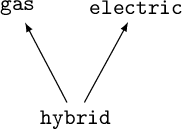
\includegraphics[height=80pt]{section6/6.1/motors.png}.
\end{center}
The functionalities the motors can deliver is given as the preorder $F$
\begin{center}
	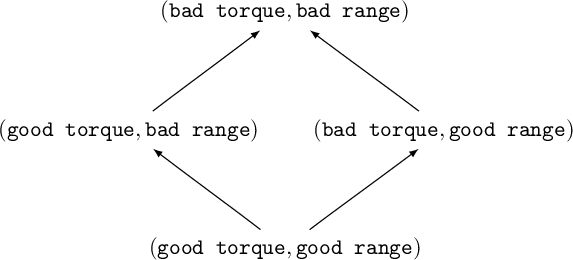
\includegraphics[height=150pt]{section6/6.1/outputs.png}.
\end{center}
The feasibility relation $\Phi: R \xslashedrightarrow{} F$ between these preorders is generated by 
$$\Phi(\mathtt{hybrid},\mathtt{(good\ torque, good\ range)}),$$
$$\Phi(\mathtt{gas},\mathtt{(bad\ torque, good\ range)}),$$
$$\Phi(\mathtt{electric},\mathtt{(good\ torque, bad\ range)}).$$

We want to model the fact that it is uncertain whether the team can provide the hybrid motor. To this end we consider collections of resources. For example, to express that the team can promise to deliver the gas motor or the hybrid motor, but they don't know which, we would use the collection $\{\mathtt{gas},\mathtt{hybrid}\}$. Such collections may as well be lower sets since the team can always include any better resources in its promise, because it just has to deliver one of the indicated resources in the end. If the team does end up delivering one of the better resources, feasibility is preserved.

In the finite setting we can represent lower sets by antichains by taking maximal elements. Thus the collection $\{\mathtt{gas},\mathtt{hybrid}\}$ becomes an antichain $(\mathtt{gas})$ which generates the original lower set by taking its lower closure. We interpret this as the promise of the team to deliver $\mathtt{gas}$ or better.

We can list all the possible promises the team can make and order them by $A \rightarrow B$ iff $\downarrow A \sub \downarrow B$:
\begin{center}
	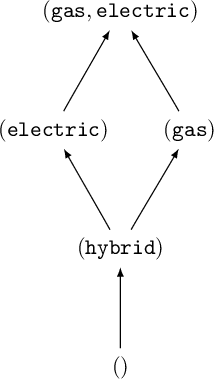
\includegraphics[width=120pt]{section6/6.1/anti_motors.png}.
\end{center}
This ordering reflects both the values of the resources and the specificity of the promise. For example, a promise of ($\mathtt{electric}$ or better) is superior to the promise of ($\mathtt{gas}$ or $\mathtt{electric}$ or better) because the former is more specific. Note that a promise of an element in the empty set is promising the impossible, and hence is better than any other promise.

We can do the same transformation to the functionalities
\begin{center}
	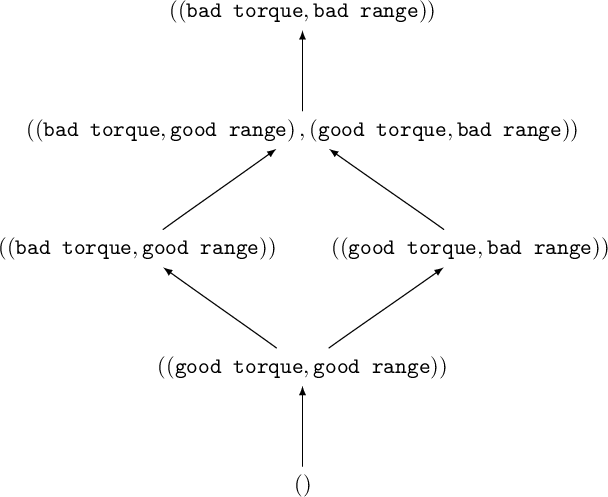
\includegraphics[width=260pt]{section6/6.1/anti_outputs.png}.
\end{center}
The uncertainty here is inherited from that in the choice of motor. If the motor team doesn't know if they can implement the hybrid design, then the other teams also don't know whether the combination of $\mathtt{(good\ torque, good \ range)}$ will be possible.

We can now express feasibility on this higher level as follows. We want a pair of collections to be feasible iff the promise of a resource in the source implies the promise of a functionality in the target. For this to work there has to be a functionality obtainable in the target, regardless of which resource in the source is provided. Formally we set
$$\hat\Phi(A,B) \iff  \forall r \in \downarrow A \: \exists f \in \downarrow B : \Phi(r,f).$$
This is again a feasibility relation since `for all' is closed under taking subsets and `exists' under taking supersets. Observe that by monotonicity of $\Phi$ we in fact have 
$$\hat\Phi(A,B) \iff \forall r \in \downarrow A \: \exists f \in \downarrow B : \Phi(r,f) \iff \forall r \in A \: \exists f \in B : \Phi(r,f).$$

Instead of extending an existing feasibility relation in this way, we could also directly define feasibility on the collections. For example, for the induced relation we have 
$$\hat\Phi((\mathtt{gas}), \mathtt{(bad\ torque, good\ range)}),$$
$$\hat\Phi((\mathtt{electic}), \mathtt{(good\ torque, bad\ range)}),$$
$$\hat\Phi((\mathtt{gas},\mathtt{electic}), \mathtt{(bad\ torque, good\ range), (good\ torque, bad\ range)}).$$
However,if we directly declare feasibility we could also set 
$$\Omega((\mathtt{gas}), \mathtt{(bad\ torque, good\ range)}),$$
$$\Omega((\mathtt{electic}), \mathtt{(good\ torque, bad\ range)}),$$
$$\Omega((\mathtt{gas},\mathtt{electic}), \mathtt{(bad\ torque, bad\ range)}).$$
In particular, 
$$\Omega((\mathtt{gas},\mathtt{electic}), \mathtt{(bad\ torque, good\ range), (good\ torque, bad\ range)}) = \mathtt{false}.$$

This choice could model some dependency that is not reducible to feasibility at the lower level. Maybe, if it is unknown whether $\mathtt{gas}$ or $\mathtt{electric}$ will be provided it is not possible to guarantee either $\mathtt{(bad\ torque, good\ range)}$ or $\mathtt{(good\ torque, bad\ range)}$ because a chassis that could fit both motors inevitably gives  $\mathtt{(bad\ torque, bad\ range)}$.

The relation $\Omega$ cannot be induced since we know that its values on the singletons $\mathtt{gas}$ and $\mathtt{electric}$ are the same as those of $\hat\Phi$. If $\Omega$ were induced by $\omega$, then $\omega$ must agree with $\Phi$ on the singletons. But in that case $\Omega = \hat\omega= \hat\Phi$, a contradiction. This shows that we can capture effects by declaring feasibility on this higher level that are not reducible to feasibility on the lower level.\\

Next we consider the choice structure on the source: 
\begin{center}
	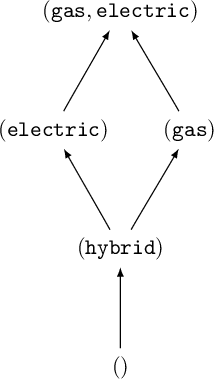
\includegraphics[width=120pt]{section6/6.1/anti_motors.png}.
\end{center}
The motor team can combine their promises. Let $A$ and $B$ represent two promises. The team can promise ($A$ or $B$), that is they promise that the resource will lie in $A$ or better, or in $B$ or better, but they are not specifying which. This is they same as promising a resource in $\downarrow A \cup \downarrow B$, which is again a lower set. The antichain that corresponds to this is $\max(\downarrow A \cup \downarrow B)$, which is the same as $\max(A \cup B)$ since $\downarrow A \cup \downarrow B = \downarrow(A \cup B)$ and $\max(\downarrow X) = \max(X)$.

For example, if the team promises $\mathtt{electric}$ or better, or $\mathtt{gas}$ or better, this is the same as promising  $(\mathtt{gas},\mathtt{electric})$ or better.

On the other hand, the motor team could combine promises in a different way. They could stipulate that we as managers get to chose between which promise ($A$ or $B$) they must fulfill. Representing this formally requires another level of choice: We as managers promise to chose among as set of promises. For example, we say that we will choose among $\{(\mathtt{electric}), \mathtt{(gas,electric)}\}$. These sets may as well be upper sets, since adding more options is good for us as managers, and at the same time adding less specific promises doesn't constrain the team either. Again we can represent the upper sets as antichains by taking minima. We order this collection by $A \rightarrow B$ iff $\uparrow A \supseteq \uparrow B$: 
\begin{center}
	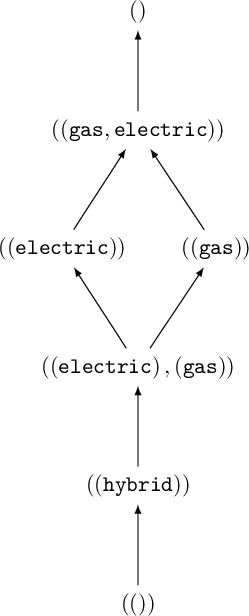
\includegraphics[width=120pt]{section6/6.1/anti_anti_motors.png}.
\end{center}
This order takes into account the specificity of our promise as well as the values of the team's promises they contain.

By the interpretation we've set up so far, the team giving us as managers the choice between which promise they need to fulfill corresponds to unioning the represented upper sets: If $A, B$ are team promises then $(A),(B)$ are the managerial promises that correspond to them. If the team gives us as managers the choice between $(A),(B)$, this corresponds to $((A),(B))$. In general, managerial choice between existing managerial choices $M,N$ is given by $\min(\uparrow M \cup \uparrow N) = \min(M \cup N)$.

We've now expressed managerial choice, but what about team choice at this level. Let $A,B$ be managerial promises. We give the team the choice between which managerial promise we will draw from. Denote managerial choice over a set $X$ by $\mathsf{M}(X)$ and denote team choice over a set $Y$ by $\mathsf{T}(Y)$. In our formal framework we have a standard representation of choice as $\mathsf{M}(\mathsf{T}Y_1, \ldots, \mathsf{T}Y_n)$. We observe that the two types of choice should distribute over on another (the reasoning behind this will be explained elsewhere). Hence, for sets $Y_i, Z_i$ of resources we have
\begin{IEEEeqnarray*}{rCl}
	\mathsf{T}(\mathsf{M}(\mathsf{T}Y_1, \ldots, \mathsf{T}Y_n),\mathsf{M}(\mathsf{T}Z_1, \ldots, \mathsf{T}Z_m)) &=& \mathsf{M}(\{\mathsf{T}(\mathsf{T}(Y_i),\mathsf{T}(Z_j)) : 1 \leq i \leq n , 1 \leq j \leq m \}) \\
	&=& \mathsf{M}(\{\mathsf{T}(Y_i \cup Z_j) : 1 \leq i \leq n , 1 \leq j \leq m \}) 
\end{IEEEeqnarray*}
Therefore, we can write a team choice between managerial promises $A,B$ as $\min\{\max(a \cup b) : a \in A, b \in B\}$. If $A$, $B$ are singletons, this reduces to the usual team choice between two team promises.

Returning to the preorder
\begin{center}
	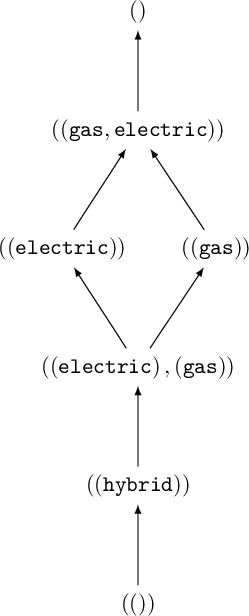
\includegraphics[width=120pt]{section6/6.1/anti_anti_motors.png}.
\end{center}
we observe that the meets of the elements are exactly managerial choice, while the joins are team choice.

We may again lift a profunctor $\Omega: \ac(R) \rightarrow \ac(F)$ from the previous level to this level as follows: A pair $(A,B)$ is feasible iff for every promise of functionalities $b \in B$, there is a promise of resources $a \in A$ such that $\Omega(a,b)$. Hence $(A,B)$ being feasible expresses that if we as managers demand a $b \in B$, there is $a \in A$ that we can select for which the teams can implement $b$ based on $a$. Formally

$$\tilde\Omega(A,B) \iff \forall b \in \uparrow B \: \exists a \in  \uparrow A: \Omega(a,b) \iff \forall b \in B\: \exists a \in  A: \Omega(a,b),$$
where the last equivalence follows by monotonicity of $\Omega$. The fact that `exists' is preserved by supersets and `for all' by subsets implies that $\tilde\Omega$ is a profunctor. 

Instead of inducing a profunctor from the lower team level, we could also directly set a profunctor at this upper level. The interpretation for setting $(A,B)$ feasible is as follows: If we as managers haven't yet decide whether to go with a specific $b \in B$, the collection of options $A$ is sufficient to guarantee that we can realize any choice we end up making. The manager is looking to keep his options open in the target and hence dependency is traveling from target to source. In the case of the teams, they want to keep options open in the source, so dependency travels in the opposite direction.\\

Let's see what types of questions we can ask at the managerial level. Let $\Psi: \ac(\ac(R)) \xslashedrightarrow{} \ac(\ac(F))$ be a profunctor at the managerial level. To start with lets consider $\Phi: R \xslashedrightarrow{} F$ generated by 
$$\Phi(\mathtt{hybrid},\mathtt{(good\ torque, good\ range)}),$$
$$\Phi(\mathtt{gas},\mathtt{(bad\ torque, good\ range)}),$$
$$\Phi(\mathtt{electric},\mathtt{(good\ torque, bad\ range)}).$$
The induced feasibility $\hat\Phi: \ac(R) \rightarrow \ac(F)$ on the team level is


The induced feasibility relation $\tilde\hat\Phi: \ac(\ac(R)) \rightarrow \ac(\ac(F))$ on the managerial level is



\newpage
\printbibliography

\end{document}
